\documentclass[a4paper]{article}

%% Language and font encodings
\usepackage[english]{babel}
\usepackage[utf8x]{inputenc}
\usepackage[T1]{fontenc}
\usepackage{multicol}
\usepackage{tikz}
\usepackage{array}
\usepackage{siunitx}
\usepackage{longtable}
\usepackage{tabularx,ragged2e, booktabs,caption}
\usepackage{float}
\usepackage{comment}
\usepackage{gensymb}
\usepackage{setspace}
\usepackage{authblk}
\usepackage{indentfirst}
\usepackage{calrsfs}


%tikz commands
\usetikzlibrary{shapes.geometric, arrows}
\tikzstyle{rect} = [rectangle, rounded corners, minimum width=2cm, minimum height=1cm,text centered, draw=black]
\tikzstyle{squ} = [rectangle, rounded corners, minimum width=2cm, minimum height=2cm, text centered, draw=black]
\tikzstyle{arrow} = [thick,->,>=stealth]
\tikzstyle{arrow} = [thick,->,>=stealth]
%% Sets page size and margins
\usepackage[a4paper,top=3cm,bottom=2cm,left=3cm,right=3cm,marginparwidth=1.75cm]{geometry}

%% Useful packages
\usepackage{amsmath}
\usepackage{amssymb}
\usepackage{graphicx}
\usepackage[colorinlistoftodos]{todonotes}
\usepackage[colorlinks=true, allcolors=blue]{hyperref}

\title{An Age Structured Model of the Impact of Buffelgrass on Saguaro Cacti and their Nurse Trees}
%\affiliation{The University of Texas Rio Grande Valley}{FIRSTAFF}
\author[1]{Lucero Rodriguez-Rodriguez}
\author[2]{Erin Stafford}
\author[3]{Anna Williams}
\author[4]{Brian Wright}
\author[5]{Christopher Kribs}
\author[6]{Karen Rios-Soto}
\affil[1]{University of Texas Rio Grande Valley}
\affil[2]{Tulane University}
\affil[3]{University of Texas at Austin}
\affil[4]{University of Redlands}
\affil[5]{University of Texas at Arlington}
\affil[6]{University of Puerto Rico at Mayaguez}

\begin{document}
\maketitle

\begin{abstract}
The saguaro cactus (Carnegiea gigantea), a keystone species in the Sonoran Desert, has faced population decline in recent years. The immediate threat to the saguaro cactus is the increase in wildfires fueled by the invasive species buffelgrass (Pennisetum ciliare). The increasing rate of wildfires could result in the collapse of the Sonoran Desert ecosystem. A stage structured model is used to capture interactions between saguaro cacti, their nurse trees, and buffelgrass. In order to accurately model the impact of buffelgrass, the interactions between the saguaro growth stages, juvenile and adult, with the nurse trees, called the foothills palo verde (Parkinsonia microphylla), is studied. The later introduction of buffelgrass to the model demonstrates its influence on the natural life cycles of the saguaro and nurse tree populations. This model consists of a system of non--linear ordinary differential equations which considers commensalism between juvenile saguaros and their nurse trees and their eventual competition as juveniles mature to adulthood. The analysis of this system includes qualitative analysis of the equilibria of the system as well as a numerical analysis of the sensitivity of key parameters. In the interest of preserving the saguaro cactus population, this system will provide insight into the effectiveness of current mitigation strategies. 
\end{abstract}

\section{Introduction}
\subsection{The Saguaro Cactus}
As a keystone species of the Saguaro National Park the saguaro cactus, or {\it{Carnegiea gigantea}}, serves not only as an icon of the national park, but also as a habitat and food source for many other species in the region \cite{keystoneDrezner}. Therefore, changes in the saguaro cactus population indicates the health of the  ecosystem \cite{keystoneDrezner}. Aside from the substantial ecological impact of saguaros, the cactus is also important for the tourism industry, with tourism to the Saguaro National Park resulting in a cumulative economic benefit of \$66.5 million  for Tucson, Arizona alone \cite{tourism}. Furthermore, the saguaro also has cultural significance to the Papago and Pima nations, who have historically relied on the plant for food, drink, and religious traditions \cite{keystoneDrezner}.\\

The saguaro cactus is a slow--growing, perennial plant that has been recorded to have a lifespan of 125 to 175 years and a maximum height of over 18 meters. Saguaros reproduce through cross pollination with other saguaros, however, they are not able to reproduce until they are 30 to 45 years of age. Most fragile in the early stages of growth, saguaro seeds flourish during infrequent weather patterns such as mild winters and summers, followed by increased rainfall. An example of their sensitivity can be noticed from past population bursts that have been linked to the subtle weather fluctuations associated with volcanic activity and El Ni\~{n}o \cite{volcano}. Since population bursts are observed from subtle weather changes, it can be inferred that the saguaro cactus reproduction is very sensitive to weather. This makes the saguaro population susceptible to the slightest weather fluctuations. Due to a long life span and slow growth many of the effects of population changes are not realized for decades or longer \cite{85yr}.
\begin{figure}[H]
\hspace{-2cm}
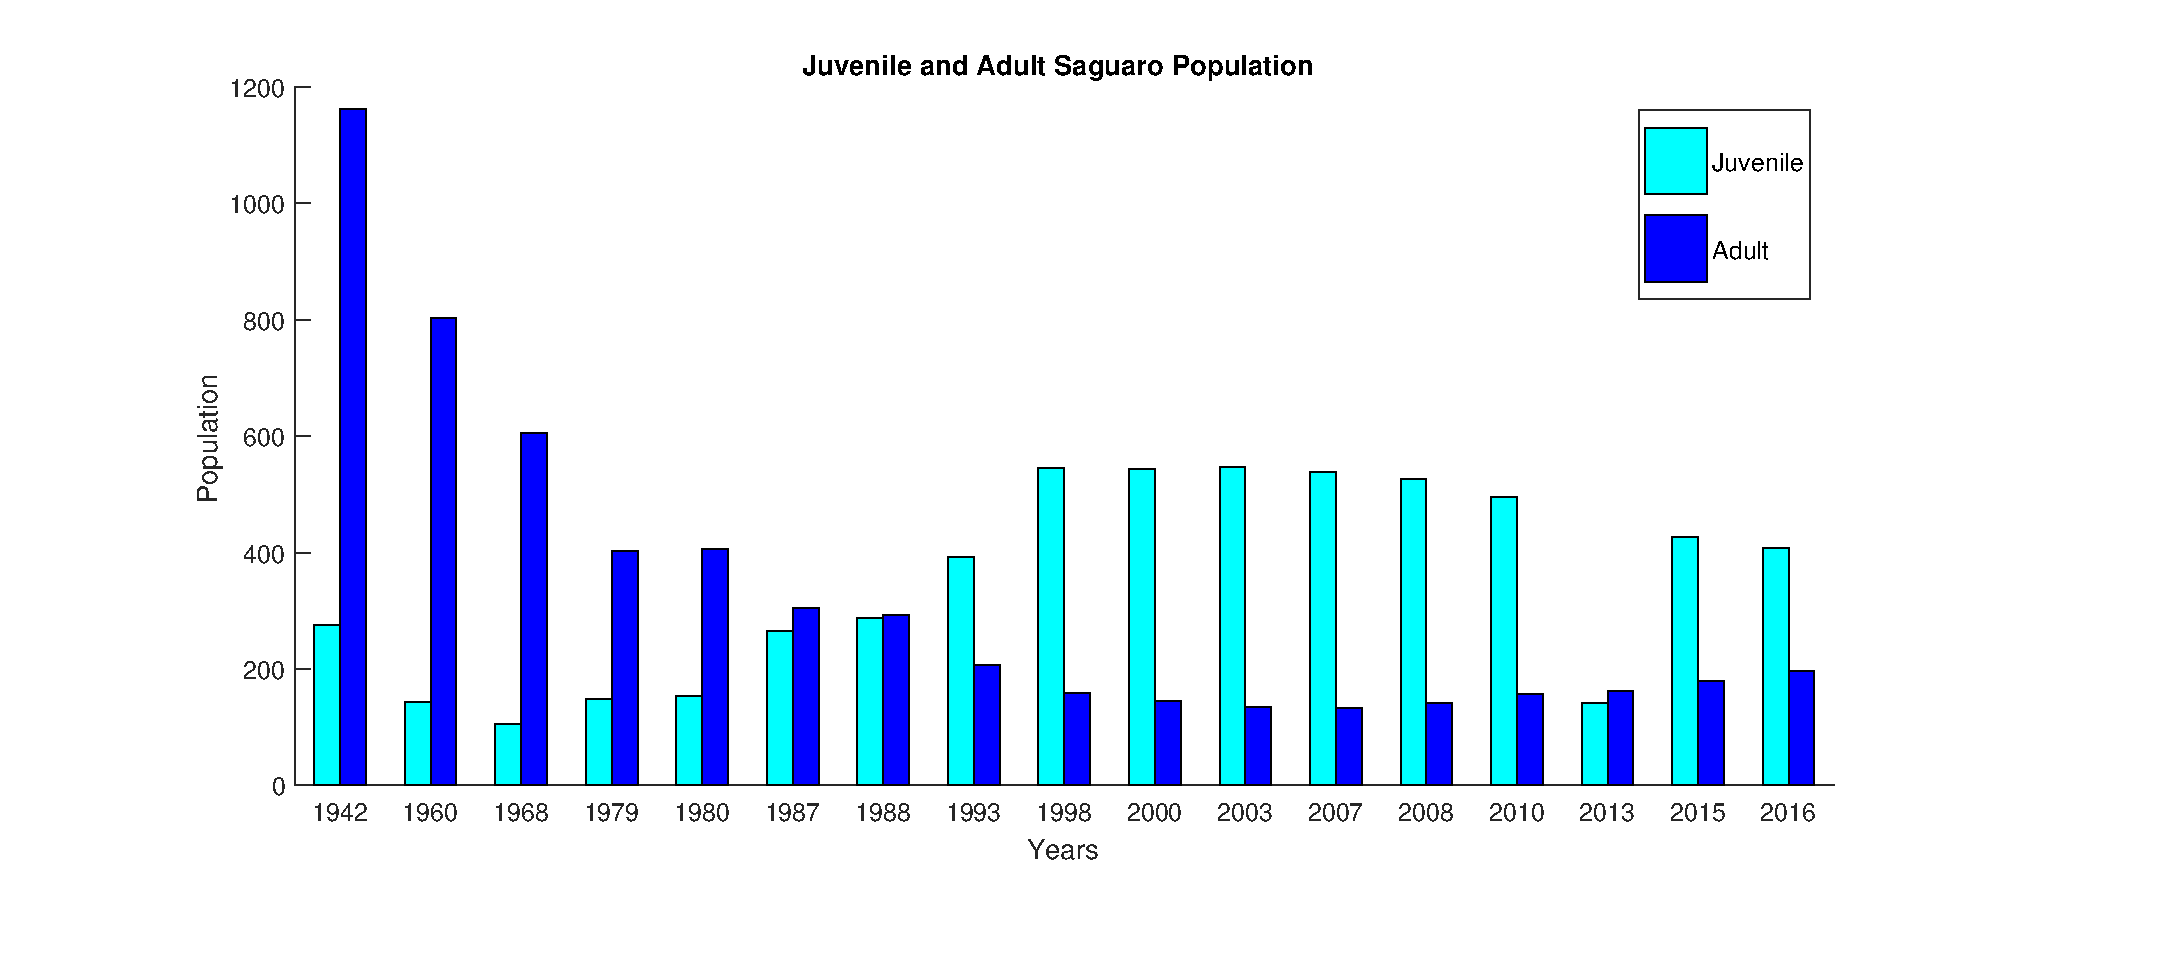
\includegraphics[scale=.55]{populationData.eps}
\caption{From data provided by Orem et.al., the changes in the distribution of adult and juvenile saguaro populations from 1942 to 2015 can be seen \cite{OrumData}. It should be noted that there is a discrepancy in the reported data in 2013.}
\label{fig:PopData}
\end{figure}
\subsection{Palo Verdes, Nurse Trees of the Saguaro Cacti}
The establishment and growth of young saguaros also depends on their nurse trees. Under their canopies, trees create a microclimate that is cooler in the summer and warmer in the winter. Nurse trees also help to protect saguaros from foraging animals and strong winds. Although saguaros can establish in the open, their likelihood to survive as a seedling is greatly increased under a nurse tree. The preference to shade results in an increased likelihood of a saguaro growing under a tree and there is a possibility of saguaro clusters around the base of trees. The most common nurse tree is the foothills palo verde, or {\it{Cercidium microphyllum}} \cite{DreznerNurses}. The foothills palo verde is a small tree with maximum height of around 7.92 meters and can live for more than 100 years. The palo verde reproduces both sexually and asexually, however, due to animal consumption and water availability only 1.6\% of all seedlings that are germinated survive, resulting in a low yearly recruitment rate for the species \cite{paloVerdeFacts}. 
\subsection{Buffelgrass}
Although saguaros are susceptible to many natural causes of death, such as freezing, drought, small animal consumption, and bacterial necrosis; the largest threat to the population is currently wildfire caused by buffelgrass \cite{Orum}. Figure \ref{fig:PopData} was constructed by previously recorded saguaro census data \cite{Orum,OrumData}. The figure shows a gradual decline in the population of both adult saguaros and juvenile saguaros starting from 1942. As a source for cattle feed and erosion control, buffelgrass was first introduced to the state of Arizona in the 1930's and was first identified in Saguaro National Park in 1989 \cite{NPSbuffel}. Buffelgrass is a perennial invasive grass that can reproduce sexually or asexually, and its seeds are viable for up to 4 years before being germinated. Fluffy and nearly weightless, buffelgrass seed spread is facilitated by wind, water, and animal fur. Furthermore, germination can occur in a range of temperatures from 50$^{\circ}$F to 104$^{\circ}$F, requires about 0.124 inches of rain over two days, and at any time of year. Once germinated, seeds mature in about 18 months, and adults can reproduce within 6 weeks. Also, in the desert regions of Arizona, buffelgrass has no natural predators, meaning that removal is limited to the manual pulling of the plants by volunteers or chemical spraying, which is only viable for a couple weeks in the rainy season when the plants are green. Buffelgrass resilience has lead to an annual population increase of 35.5\% in Saguaro National Park \cite{NPSbuffelFact}. As an invasive species, buffelgrass is able to out-compete many native species in the Sonoran Desert. Moreover, buffelgrass is a fire-adapted species, meaning it can quickly reemerge after wildfire and provide fuel so that the fires burn longer and cover more area. Buffelgrass helps the quick spread of fire, which kills native species and leaves available space for the buffelgrass to invade at a faster rate than the native species \cite{buffelFireInfo}.\\

In the following sections, a mathematical model is formulated to look at the interactions of saguaros and their nurse trees and the influence of buffelgrass on the system. Equilibria and sensitivity analyses will be preformed on the model. The purpose of this model is to predict the longterm effects of buffelgrass can have the saguaro population as well as if any resulting population decline can be reduced through the control of the buffelgrass population.\\

\section{Formulating the Method}
In order to predict the impact of buffelgrass on the saguaro cactus, as well as the palo verde nurse tree, the dynamics of the saguaro and nurse tree populations is modeled with and without the inclusion of buffelgrass. This design will reveal the true impact of buffelgrass on the cactus and trees and allow us to analyze the extent of the buffelgrass wildfire damage. The model without buffelgrass serves to demonstrate the natural interaction of the saguaro cactus and the nurse trees. The introduction of buffelgrass to the model exhibits the extent of the damage caused by buffelgrass wildfires. These models will be systems of non--linear ordinary differential equations (ODEs) that represent the basic interactions between the populations. The inclusion of buffelgrass will predominantly reflect the effects of wildfires on saguaro cactus and their nurse trees.
\subsection{Assumptions of the Model}
Assumptions were made about the interactions between saguaros, nurse trees, and buffelgrass in order to maintain realistic dynamics and avoid unnecessary complexity.\\

The first of these assumptions is that juvenile saguaros are assumed to be cacti in the age range of 1 to 35. The range starts at age 1, because this is when a cacti's susceptibility to death due to environmental conditions is greatly reduced. The range ends at 35, because this is when cacti are able to begin reproducing. Therefore, the adult saguaro population considers those to be at reproductive age, 35, and older. Another assumption is that the natural life span of all adult saguaros is 175 years, which is the average lifespan.\\

Also, saguaros in both age groups are equally susceptible to death from conditions like extreme temperature, bacterial necrosis, and being eaten by rodents. Furthermore, the difference in the survival rates of the juvenile saguaros under nurse trees and in the open are not considered.\\

The model does not consider the effects of clustering of the adult population on the reproductive rate, since this is rarely seen. For the nurse trees, assumptions include that trees are not able to out compete adult saguaros for resources. Furthermore, the only competition that juvenile saguaros face is competition over space with adult saguaros. So, competition between juvenile saguaros and buffelgrass is not included. Competition between nurse trees and buffelgrass is also not included because the effects are not strong. Similarly, commensalism between adult saguaros and buffelgrass is not included because the effects do not greatly influence either species.

\subsection{The Model}
The model is formulated using the dynamics between the adult and juvenile saguaro cacti, their nurse trees, and buffelgrass. The interactions considered are given by the equations below.
\newline \newline \newline
\begin{subequations}
\begin{equation}
\displaystyle\frac{dS_j}{dt}= rS_a\cdot \text{max}\left\lbrace0,\left(1-\displaystyle\frac{\epsilon S_j + S_a}{k_1+b T}\right) \right\rbrace - \gamma S_j - \mu_j S_j - \theta_j B S_j
\end{equation}

\begin{equation}
\displaystyle\frac{dS_a}{dt} = \gamma S_j -\displaystyle\frac{\alpha_1}{k_2}S_a T - \mu_a S_a - \theta_a B S_a
\end{equation}

\begin{equation} \label{eqBuffel}
\displaystyle\frac{dS_T}{dt} = \phi T\left(1 - \displaystyle\frac{T + \sigma S_a}{k_2}\right) - \theta_T B T
\end{equation}

\begin{equation}
\displaystyle\frac{dB}{dt} =\omega B \left(1-\displaystyle\frac{B}{k_3}\right) - \mu_B B
\end{equation}
\end{subequations}

The growth of the juvenile saguaro population, $S_j$, from the reproduction of the adult saguaros, $S_a$, is best captured with a logistic growth term, given by
\begin{equation}\label{eq:juvenilegrowth}
rS_a\left(1 - \displaystyle\frac{\epsilon S_j + S_a}{k_1 +b T}\right)
\end{equation}\\
The juvenile--adult interaction, equation \ref{eq:juvenilegrowth}, represents the rate that new juvenile saguaros enter the population. The term $r$ represents the number of seeds that germinate and survive to one year of age per adult saguaro. The term,$$ \displaystyle\frac{\epsilon S_j + S_a}{k_1 +bT}$$ represents the proportion of space available for new juveniles to take root, including free space not taken by adults and space under nurse trees. The numerator, $\epsilon S_j + S_a$ is the space that is already taken up by juvenile and adult saguaros. The parameter $\epsilon$ converts juveniles to adults in terms of space, so that the carrying capacity term will be scaled to adults only. In the denominator, $k_1+bT$ represents the benefit nurse trees provide to juvenile saguaros by increasing their carrying capacity. Here, $k_1$ is the carrying capacity of adult saguaros in open space and $b T$ is the average number of saguaros one nurse tree can support. Therefore, nurse trees increase the number of juveniles that can survive in an area. Since this term has the possibility to be negative, we take the maximum value between zero and the term described previously for the biological application. Furthermore,$\gamma$ is the rate at which juveniles mature. Here it is assumed that juveniles become adults when they begin to reproduce.\\

For the adult population, $\mu_a$ represents the death rate, and the rate at which adult saguaros die due to competition with trees for resources is $\displaystyle\frac{\alpha_1}{k_2}.$ It is assumed that $\alpha_1$ is nearly zero since the possibility of a nurse tree out competing an adult saguaro is rare.\\

The dynamics of the tree population include natural germination and death rates, given in $\phi.$ The rate that nurse trees reach their carrying capacity, $k_2$, is given by $\phi T\displaystyle\frac{T}{k_2}.$ The term for the competition between adult saguaros and trees, $\rho S_a T$, can be rewritten as $\phi T\displaystyle\frac{\sigma S_a}{k_2}$, where $\sigma$ is a proportion of the carrying capacity, and is dimensionless, that is given by $\sigma = \displaystyle\frac{\rho}{\phi}k_2$\\

Since the main effect of buffelgrass on native species in regions where it has invaded is the propagation of wildfire, the dynamics of buffelgrass interacting with native populations in the terms of competition or commensalism are neglected.\\

The parameters $\theta_i$ ($i$= $j$, $a$, or $T$) represents the effect of buffelgrass-related wildfire. Thus, the terms in the saguaro and nurse tree equations, $\theta_j B S_j$, $\theta_a B S_a$, and $\theta_T B T$ are the mechanism for the death of these species due to wildfires. The $\theta$'s are dependent on the density of buffelgrass and describe the frequency of wildfires in the area under study.\\

It is assumed that the buffelgrass equation grows logistically, that is $\omega B \left(1-\displaystyle\frac{B}{k_3}\right),$ where $\omega$ is natural growth rate. When implementing mitigation strategies, such as seasonal chemical spraying, $\omega$ will be decreased. The term for the space already occupied by buffelgrass is $\displaystyle\frac{B}{k_3}$, $k_3$ is the carrying capacity. Constant effort harvesting is also incorporated in the model, with $\mu_B B$  representing efforts by volunteers to reduce the buffelgrass population through the manual pulling of buffelgrass. Thus, $\mu_B$ is the harvesting rate.\\

The system of equations representing the population dynamics described above can also be represented in a flow chart diagram.
\begin{figure}[H]
\begin{figure}
    \begin{center}
    \tiny{
        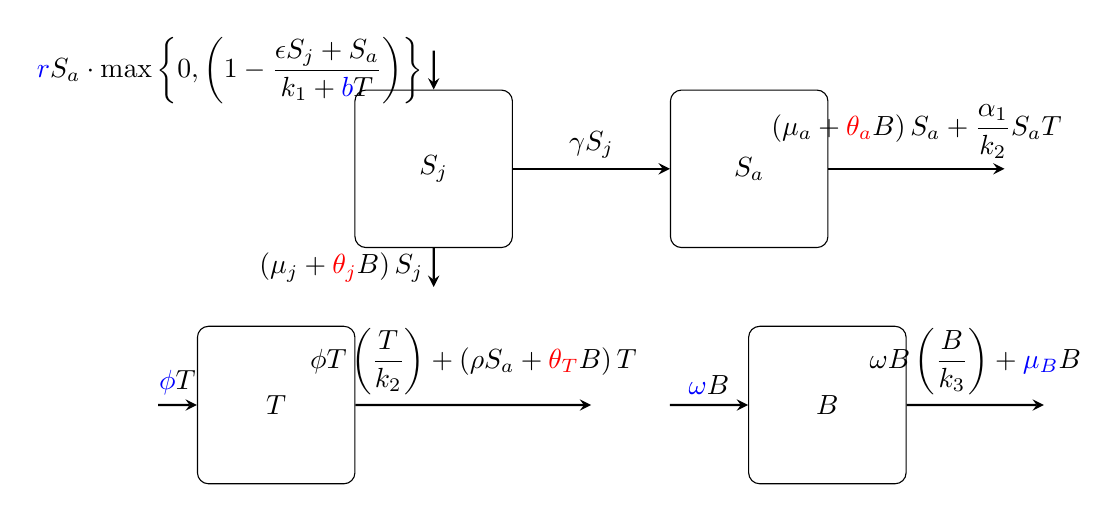
\begin{tikzpicture}[scale = 0.5,node distance=1cm]
        \node (eq1) [squ, xshift = -4cm,yshift=-1cm] {$S_j$};
        \node (eq2) [squ, right, xshift=-1cm, yshift=-1cm] {$S_a$};
        \draw [arrow] (eq1) -- node[anchor=south] {$\gamma S_j$}(eq2);
        \node (eq3) [squ, xshift=-6cm, yshift=-4cm] {$T$};
        \node (eq4) [squ, xshift = 1cm, yshift = -4 cm]{$B$};
        \coordinate (plain1) at (-8,1) {};
        \draw [arrow] (plain1)--node[anchor=east]{$\textcolor{blue}{r} S_a\cdot\text{max}\left\lbrace0,\left(1-\displaystyle\frac{\epsilon S_j + S_a}{k_1 + \textcolor{blue}{b} T}\right)\right\rbrace$}(eq1);
        
        \coordinate (plain2) at (-8,-5){};
        
        \draw[arrow](eq1)--node[anchor=east]{$\left(\mu_j + \textcolor{red}{\theta_j} B\right)S_j$}(plain2);
        
        \coordinate (plain3) at (6.5,-2){};
        \draw [arrow](eq2)--node[anchor=south]{$\left(\mu_a + \textcolor{red}{\theta_a} B\right)S_a + \displaystyle\frac{\alpha_1}{k_2} S_a T$}(plain3);
        
        \coordinate(plain4) at (-4,-8){};
        \draw [arrow](eq3)--node[anchor=south]{$\phi T \left( \displaystyle\frac{T}{k_2}\right) + \left(\rho S_a + \textcolor{red}{\theta_T} B\right) T$}(plain4);
        
        \coordinate(plain5) at (-15,-8){};
        \draw[arrow](plain5)--node[anchor=south]{$\textcolor{blue}{\phi} T$}(eq3);
        
        \coordinate (plain6) at (-2,-8){};
        \draw[arrow](plain6) -- node[anchor = south]{$\textcolor{blue}{\omega} B$}(eq4);
        
        \coordinate(plain7) at (7.5,-8){};
        \draw[arrow](eq4) -- node[anchor = south]{$\displaystyle\omega B\left(\frac{B}{k_3}\right) + \textcolor{blue}{\mu_B} B$}(plain7);
        \end{tikzpicture}
        }
    \end{center}
    \label{fig:tikz}
\end{figure}
\caption{Flow chart diagram representing interactions between juvenile and adult saguaros, and nurse trees with the effects of buffelgrass}
\label{fig:ModelWithBuffel}
\end{figure}

\subsection{The Model without Buffelgrass}
In order to observe the dynamics of the saguaro and nurse tree populations of the model before the invasion of buffelgrass, a case of the model with $B = 0$ is considered.

\begin{subequations}
\begin{equation}\label{SjNobg}
\displaystyle\frac{dS_j}{dt}= rS_a\cdot \text{max}\left\lbrace0,\left(1-\displaystyle\frac{\epsilon S_j + S_a}{k_1+b T}\right)\right\rbrace - \gamma S_j - \mu_j S_j
\end{equation}

\begin{equation}
\displaystyle\frac{dS_a}{dt} = \gamma S_j -\displaystyle\frac{\alpha_1}{k_2}S_a T - \mu_a S_a
\end{equation}

\begin{equation}
\displaystyle\frac{dT}{dt} = \phi T\left(1 - \displaystyle\frac{T}{k_2}\right) - \rho S_a T
\end{equation}
\end{subequations}

From these equations, pre-buffelgrass values for equilibria can be found and compared to those after buffelgrass becomes incorporated into the ecosystem.The flow chart diagram for the case without buffelgrass is given in Figure \ref{fig:OriginalModel}.

\begin{figure}[H]
\begin{figure}[H]
    \begin{center}
        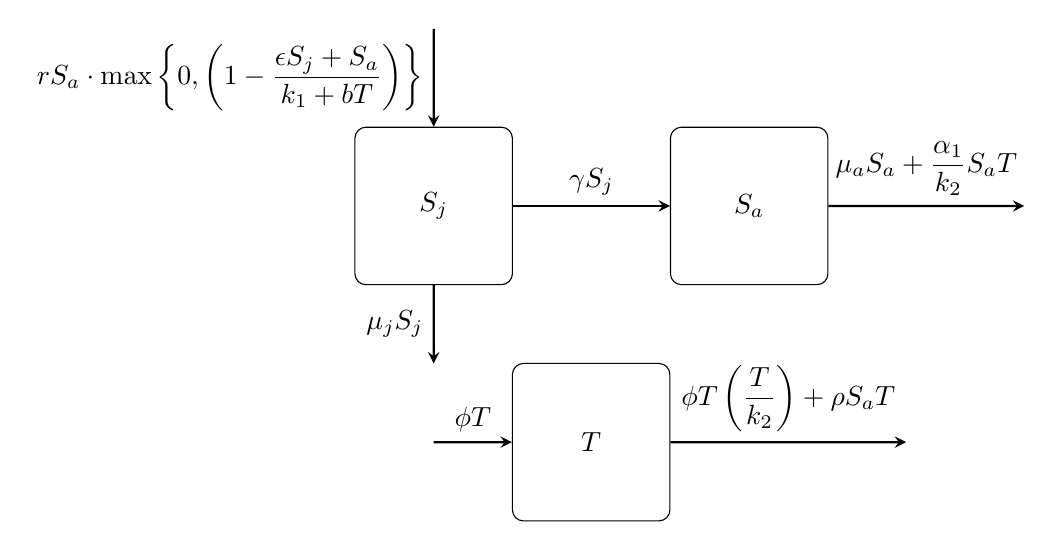
\begin{tikzpicture}[node distance=2cm]
        \node (eq1) [squ, xshift = -2cm,yshift=-3cm] {$S_j$};
        \node (eq2) [squ, right, xshift=1cm, yshift=-3cm] {$S_a$};
        \draw [arrow] (eq1) -- node[anchor=south] {$\gamma S_j$}(eq2);
        \node (eq3) [squ, xshift=0cm, yshift=-6cm] {$T$};
        \coordinate (plain1) at (-2,-0.75) {};
        \draw [arrow] (plain1)--node[anchor=east]{$r S_a\cdot\text{max}\left\lbrace0,\left(1-\displaystyle\frac{\epsilon S_j + S_a}{k_1 + b T}\right)\right\rbrace$}(eq1);
        \coordinate (plain2) at (-2,-5){};
        
        \draw[arrow](eq1)--node[anchor=east]{$\mu_j S_j$}(plain2);
        
        \coordinate (plain3) at (5.5,-3){};
        \draw [arrow](eq2)--node[anchor=south]{$\mu_a S_a + \displaystyle\frac{\alpha_1}{k_2} S_a T$}(plain3);
        
        \coordinate(plain4) at (4,-6){};
        \draw [arrow](eq3)--node[anchor=south]{$\phi T \left( \displaystyle\frac{T}{k_2}\right) + \rho S_a T$}(plain4);
        
        \coordinate(plain5) at (-2,-6){};
        \draw[arrow](plain5)--node[anchor=south]{$\phi T$}(eq3);
        \end{tikzpicture}
    \end{center}
    \label{fig:tikz}
\end{figure}
\caption{Flow chart diagram of the saguaro model without buffelgrass}
\label{fig:OriginalModel}
\end{figure}

\section{Analysis of the Model}
\subsection{Equilibria without Buffelgrass}
There are five potential possible equilibrium points for this model. Three of which describe the extinction condition for both or one species. The other equilibrium points describe coexistence criteria. Not all equilibrium always exist, so conditional statements are defined for coexistence.\\

Let the equilibrium points be denoted by \newline
$$E_k = (S_{jk}^*, S_{ak}^*, T_k^*)$$

\subsubsection{Total Extinction}
By setting equation 3c equal to zero, the an equilibrium value of $T^*$ is found to be 
\begin{equation*}
T^* = 0
\end{equation*}
Plugging $T^* = 0$ into equation 3b and setting the new equation equal to zero produces:
\begin{equation*}
S_j^*(S_a) = \displaystyle\frac{\mu_a}{\gamma} S_a^*
\end{equation*}
From here, substituting $T^*(S_a)$ and $S_j^*(S_a)$ into equation 3a gives 
\begin{equation*}
S_a^* = 0
\end{equation*}
as one of the equilibrium values of $S_a$, which also means $S_j^* = 0$. Using $T^*=0$, the total extinction equilibrium is found to be
$$E_1 = (S_j^* , S_a^* , T^*) =  (0 , 0 , 0)$$


\subsubsection{Cacti Exclusion Equilibrium}
The cacti exclusion equilibrium refers to the point with cactus population dies out, or (0 , 0 , $T^*$). From the previous section, if $S_a^* = 0$, then $ S_j^* = 0$. To find the equilibrium value of $T$, when there is not total extinction, equation 3c is set equal to zero. This gives 
\begin{equation*}
T^*(S_a) = k_2\left(1-\displaystyle\frac{\rho}{\phi}S_a\right)
\end{equation*}
From the above equation, it is important to note that in order for $T^*(S_a) > 0$ to be true, $S_a^*<\displaystyle\frac{\phi}{\rho}$.  Substituting in $S^*_a = 0$ into the equation above gives $T^* = k_2$. Therefore, $$E_2 = (S_j^* , S_a^* , T^*) =(0 , 0 , k_2)$$

\subsubsection{Nurse Tree Exclusion Equilibrium}
The nurse tree exclusion equilibrium refers to the point with nurse tree population dies out, such that ($S_j^*$ , $S_a^*$ , 0). Using the equilibrium values $T^*$ = 0, and $S_j^*(S_a) = \displaystyle\frac{\mu_a}{\gamma} S_a^*$, it is possible to substitute these values into equation 3a to get $$S_a^* = r\left(1 - \left(\displaystyle\frac{\displaystyle\frac{\epsilon\cdot \mu_a}{\gamma}S_a^* + S_a^*}{k_1}\right)\right) - \displaystyle\frac{\left(\gamma+\mu_j\right)\mu_a}{\gamma}$$

Letting $R_{d1} = \displaystyle\frac{\gamma}{\gamma+\mu_j} \cdot\displaystyle\frac{r}{\mu_a}$ and $E=\displaystyle\frac{\epsilon \cdot \mu_a}{\gamma} $ gives 
\begin{equation*}
S_a^* = \displaystyle\frac{k_1 \left(1 - \displaystyle\frac{1}{R_{d1}}\right)}{E+1}
\end{equation*}

Next, plugging in the newly found value of $S_a^*$ into the definition of $S_j^*$ and using $T^* = 0$ produces:
$$E_3 = (S_j^*,S_a^*,T^*) = \left(\left(\displaystyle\frac{\mu_a}{\gamma}\right) \displaystyle\frac{k_1}{E+1} \left(1 - \displaystyle\frac{1}{R_{d1}}\right) \text{ , }\displaystyle\frac{k_1}{E+1} \left(1 - \displaystyle\frac{1}{R_{d1}}\right)\text{ , }0\right)$$
Thus, $E_3$ exists if $R_{d1} > 1$.

\subsubsection{Coexistence}
The coexistence equilibrium represents when all species live in the same environment and share the same space and resources. 
Hence, by ($T^* \neq 0$):

Let $\eta_a^* = \displaystyle\frac{S_a^*}{\phi/\rho}$, thus $0 < \eta_a^* < 1$ Then
\begin{equation*}
T^*(\eta_a^*) = k_2( 1- \eta_a^*) \rightarrow T^* > 0 \textbf{ iff } \displaystyle\frac{S_a^*}{\phi/\rho} < 1
\end{equation*}
\begin{equation*}
S_j^*(\eta_a^*) = \displaystyle\frac{\phi}{\rho}\left(\displaystyle\frac{\mu_a + \alpha}{\gamma}\right)\eta_a^* -  \displaystyle\frac{\phi\alpha}{\rho\gamma}\eta_a^{2*}
\end{equation*}
Now, to solve for $\eta_a^*$: %and let $R_{d2} = \displaystyle\frac{r}{\mu_a+\alpha}\cdot\frac{\gamma}{\gamma + \mu_j}$:
\begin{equation*}
0 = r\displaystyle\frac{\phi}{\rho}\eta_a^*\left[1 - \frac{\frac{\phi}{\rho}(\eta_a^*(\frac{\epsilon\mu_a}{\gamma} + 1 + \frac{\alpha}{\gamma}) - \eta_a^{2*}\frac{\epsilon \alpha}{\gamma})}{k_1 + bk_2(1-\eta_a^*)}\right] - \frac{\phi}{\rho}\left(\frac{1}{R_{d2}} - \frac{\alpha\eta_a^*}{\mu_a R_{d1}}\right)
\end{equation*}
%(\gamma + \mu_j)\left(\frac{(\mu_a+\alpha)S_a}{\gamma} - \displaystyle\frac{\alpha\rho S_a^2}{\gamma\phi}\right)
If $E = \frac{\mu_a\epsilon}{\gamma}$The equation then reduces to:
\begin{equation*}
0 = \left(\displaystyle\frac{\alpha\phi\epsilon}{\rho\gamma} - \frac{bk_2\alpha}{\mu_aR_{d1}}\right)\eta_a^2 + \left[(k_1 + bk_2)\displaystyle\frac{\alpha}{\mu_a R_{d1}} - bk_2\left(1-\frac{1}{R_{d2}}\right) - \frac{\phi}{\rho}\left(1 + E + \frac{\epsilon \alpha}{\gamma}\right)\right]\eta_a^*+ (k_1 + bk_2)\left(1-\frac{1}{R_{d2}}\right)
\end{equation*}
Then, let
\begin{equation*}
\tau_1 =  \left(\displaystyle\frac{\alpha\phi\epsilon}{\rho\gamma} - \frac{bk_2\alpha}{\mu_aR_{d1}}\right)\text{, }
\tau_2 = \left[(k_1 + bk_2)\displaystyle\frac{\alpha}{\mu_a R_{d1}} - bk_2\left(1-\frac{1}{R_{d2}}\right) - \frac{\phi}{\rho}\left(1 + E + \frac{\epsilon \alpha}{\gamma}\right)\right] \text{, and }
\tau_3 = (k_1 + bk_2)\left(1-\frac{1}{R_{d2}}\right)
\end{equation*}
such that
\begin{equation*}
f(\eta_a^*) = \tau_1 \eta_a^{2*} + \tau_2 \eta_a^* + \tau_3
\end{equation*}
Notice that $f(0)$ is equal to $\tau_3$ then $\tau_3>0$ \textbf{iff} $R_{d2} > 1$. If $f(1) = k_1\left(1 - \frac{1}{R_{d1}}\right) - \frac{\phi}{\rho}(1 + E)$ is less than zero \textbf{iff} $\frac{\phi}{\rho} > \frac{k_1}{1+E}\left(1 - \frac{1}{R_{d1}}\right)$. Therefore, the following theorem can be concluded:

\textbf{Theorem 1} \textit{If $R_{d2} > 1$ and $\frac{\phi}{\rho} > \frac{k_1}{1+E}\left(1 - \frac{1}{R_{d1}}\right)$ then there exists at least one positive root of $f(\frac{S_a^*}{\phi/\rho}$ = 0 and there exists at least one co-existence equilibrium.}

$R_{d1} > \displaystyle\frac{bk_2\rho}{\phi E}$ then $\tau_1$,$\tau_2$,$\tau_3$ > 0, which implies that there is at least one coexistence equilibrium. 

\begin{comment}
In order for two positive roots to exist it is required that $\tau_1 > 0$, $\tau_2 > 0$, and $\tau_3 > 0$ if and only if the following conditions hold true: \newline \newline
$\phi > \rho$, this is assumed to be true since the rate of tree growth must be greater than the rate of tree out competition by the saguaro. \newline
\begin{equation*}
R_{d2} > 1
\end{equation*}
\begin{equation*}
R_{d1} > \frac{k_2 b \rho}{E\phi}
\end{equation*}
\begin{equation*}
S_a^* < \frac{\phi}{\rho}
\end{equation*}
Where $E = \displaystyle\frac{\epsilon\mu_a}{\gamma}$, $R_d1 = \displaystyle\frac{r}{\mu_a}\cdot\displaystyle\frac{\gamma}{\gamma+\mu_j}$, and $R_{d2} = \displaystyle\frac{r}{\mu_a + \alpha}\cdot\displaystyle\frac{\gamma}{\gamma + \mu_j}$.
\end{comment}
\begin{comment}

\subsection{Finding the Equilibria}
In order to solve for equilibria, we began by setting the equation $$\displaystyle\frac{dT}{dt} = 0$$\\ 
From there, it can be seen there are two possibilities, $$T^*_1 = 0 \text{ or } T^*_2 = k_2 - \alpha_2 \cdot S_a$$ 
From here, we can substitute these solutions for $T$ into another equation, say $\displaystyle\frac{dT}{dt}$. 
Using $T^*_1$ = 0 gives us: $$\displaystyle\frac{dS_a}{dt} = \gamma{_j}S_j - \mu{_a}S_a$$Further, we can solve for $S_j$ in terms of $S_a$ by setting $\displaystyle\frac{dS_a}{dt}$ = 0, giving us $$S_j^* = \displaystyle\frac{\mu{_a}S_a}{\gamma{_j}}$$Finally, we can set our last equation equal to 0, giving us $$\displaystyle\frac{dS_j}{dt} = r_1S_a(1-\displaystyle\frac{\epsilon S_j + S_a}{K_1+b T}) - \gamma{_j}S_j - \mu{_j}S_j = 0$$

Next, we can plug in our values for $T^*$ and $S_j^*$, giving us 

$$\displaystyle\frac{dS_j}{dt} =  r_1S_a(1-\displaystyle\frac{\epsilon \displaystyle\frac{\mu{_a}S_a}{\gamma{_j}} + S_a}{K_1}) - (\gamma{_j}+ \mu{_j}) \displaystyle\frac{\mu{_a}S_a}{\gamma{_j}} = 0$$

Which is satisfied by,
$S_{a_1}^*$ = 0, and $S_{a_2}^* = \displaystyle\frac{k_1 (r_1 \gamma{_j}-\mu{_a} (\gamma{_j}+\mu{_j}))}{r_1 (\gamma{_j}+\epsilon \mu{_a})}$.
Plugging these values into our definition for $\displaystyle\frac{dS_j}{dt}$, we get: $$S_{j_1} = 0 \text{ and  } S_{j_2} = \displaystyle\frac{k_1 \mu{_a} (-r_1 \gamma{_j} + \mu{_a} (\gamma{_j} + \mu{_j}))}{r_1 \gamma{_j} (\gamma{_j}+\epsilon \mu{_a})}$$
This, coupled with our $T^*$ gives us two equilibrium. The total extinction, (0,0,0), and the nurse tree extinction, ($\displaystyle\frac{k_1 \mu{_a} (-r_1 \gamma{_j} + \mu{_a} (\gamma{_j} + \mu{_j}))}{r_1 \gamma{_j} (\gamma{_j}+\epsilon \mu{_a})}$ , $\displaystyle\frac{k_1 (r_1 \gamma{_j}-\mu{_a} (\gamma+\mu{_j}))}{r (\gamma{_j}+\epsilon \mu{_a})}$ , 0).
In order to find the next equilibrium, we evaluate the other $T^*$ value we found, $T^* = k_2 - \alpha_2 S_a$.

Again, we can plug this into $\displaystyle\frac{dS_a}{dt}$ and set equal to 0 to get:
$$\displaystyle\frac{dS_a}{dt} = \gamma S_j -\displaystyle\frac{\alpha_1}{K_2}S_a (k_2 - \alpha_2 S_a) - \mu_a S_a = 0$$
We can solve this equation to get $S_j$ in terms of $S_a$, $S_j^*$ = $\displaystyle\frac{S_a (\mu_a + \displaystyle\frac{\alpha_1}{k_2} (k_2-\alpha_2 S_a)}{\gamma}$
Next, we substitute both of these points into $\displaystyle\frac{dS_j}{dt}$:

$$\displaystyle\frac{dS_j}{dt} = rS_a\cdot \text{max}\{0,(1-\displaystyle\frac{\epsilon \displaystyle\frac{S_a (\mu_a + \displaystyle\frac{\alpha_1}{k_2} (k_2-\alpha_2 S_a)}{\gamma} + S_a}{K_1+b T})\} - (\gamma + \mu_j) \displaystyle\frac{S_a (\mu_a + \displaystyle\frac{\alpha_1}{k_2} (k_2-\alpha_2 S_a)}{\gamma} = 0$$

One clear solution to this is $S_a^*$ = 0, which means that $S_j^0$ = 0, and $T^*$ = k2. Thus, another equilibrium point is the extinction of Saguaros, (0 , 0 , k2).
\end{comment}
\subsection{Analyzing the Equilibria}
Using the Jacobian of the model equations without the inclusion of buffelgrass, which is found in the appendix as Equation \ref{eq:noBuffelJacobian}, it is possible to test the stability of each equilibrium point. 

\subsubsection{Total Extinction}
The total extinction equilibrium point, $E_1$, is (0,0,0).
The Jacobian at this point is:
$$ \begin{pmatrix}
-(\gamma +\mu_j) & r & 0\\
\gamma & -\mu_a & 0\\
0 & 0 & \phi
\end{pmatrix}$$
Looking at this matrix, it is evident that $\phi$ is an eigenvalue, and $\phi$ is always positive. Therefore the equilibrium point for the extinction of all three populations is unstable.

\subsubsection{Cactus Exclusion Equilibrium}
Next, the cactus exclusion equilibrium is analyzed. From this analysis, the following theorem is produced.

\textbf{Theorem 2} \textit{If $R_{d2} = \displaystyle\frac{r}{(\mu_a+\alpha_1)}\frac{\gamma}{(\mu_j+\gamma)}<1$, then there exists one \textbf{stable} equilibrium point where the saguaros have gone extinct, $E_2$ = ($0$ , $0$ , $k_2$) } \\ \\
\textbf{Proof}
In order to test for local stability, the Jacobian matrix must be applied to the point, $E_2$ = (0 , 0 , $k_2$), giving:
$$ \begin{pmatrix}
-(\gamma +\mu_j) & r & 0\\
\gamma & -(\alpha_1+\mu_a) & 0\\
0 & -\sigma \phi & -\phi
\end{pmatrix}$$
It is evident that one eigenvalue is $\lambda = -\phi$, which is always negative.
The remaining eigenvalues can be found with the characteristic polynomial:\newline
\begin{equation*}
(\lambda + (\gamma + \mu_j))(\lambda + (\alpha_1 + \mu_a)) - r\gamma = 0
\end{equation*}
\begin{equation*}
\lambda^2 + (\alpha_1 + \mu_a + \gamma + \mu_j)\lambda + r\gamma \left(\frac{1}{R_{d2}} - 1 \right) = 0
\end{equation*}
Here it can be observed that since parameter values will always be positive, $m = (\gamma + \alpha + \mu_a + \mu_j)$ will always be positive. Additionally, $f = r\gamma\left(\frac{1}{R_{d2}} - 1\right)$ is greater than zero if and only if $R_{d2} < 1.$ Since $R_{d2} < 1$ is assumed and the analysis of the two remaining eigenvalues goes as follows:\newline
\begin{equation*}
\lambda_{2,3} = \frac{-m \pm \sqrt{m^2 - 4f}}{2}
\end{equation*}
Notice that since $m > 0$ and $f > 0$ then
\begin{equation*}
 \sqrt{m^2 - 4f}<m
\end{equation*}
Then, $\lambda_2$ and $\lambda_3$ will always be negative.

\subsubsection{Nurse Tree Exclusion Equilibrium}
The nurse tree extinction equilibrium, $E_3$, was found to be
$$S_j^* = \displaystyle\frac{\mu_a}{\gamma}\left(\frac{\gamma k_1}{\epsilon \mu_a + \gamma}\right)\left(1 - \frac{1}{R_{d1}}\right)$$
and
$$S_a^* = \left(\frac{\gamma k_1}{\epsilon \mu_a + \gamma}\right)\left(1 - \frac{1}{R_{d1}}\right)$$
such that 
$E_3$ = $\left(\displaystyle\frac{\mu_a}{\gamma}S_a^* \text{ , }  S_a^* \text{ , } 0\right)$.\\

In order for both $S_a^*$ and $S_j^*$ > 0, $R_{d1} > 1$. This condition is applied because values for $S_a^*$ and $S_j^*$ that are negative are of no interest or meaning. \newline




\textbf{Theorem 3} \textit{If $\displaystyle\frac {\phi}{\rho} < \displaystyle \frac{k_1}{1+\displaystyle\frac{\epsilon\cdot\mu_a}{\gamma}}(1-\displaystyle\frac{1}{R_{d1}}) $ and $R_{d1} > 1$, then the nurse tree extinction equilibrium, $E_3$ = ($S^*_j$ , $S^*_a$ , 0), is locally asymptotically stable.} \newline

\textbf{Proof:}\newline

Let $E = \frac{\epsilon\mu_a}{\gamma}$ and $S_{a2}^* = \displaystyle\frac{k_1}{E+1}(1-\frac{1}{R_d1})$. Assume $\displaystyle\frac {\phi}{\rho} < \displaystyle \frac{k_1}{1+E}(1-\displaystyle\frac{1}{R_{d1}}) $ and $R_d1 > 1$ :\newline

$$\begin{pmatrix}
-\frac{{\epsilon}r}{k_1}S_{a2}-({\mu_j} + {\gamma_j}) & r\left[1-(2+E)\frac{S_{a2}}{k1}\right] &  rb(1+E)\left(\frac{S_{a2}^2}{k^2_1}\right)\\

\gamma_j & -\mu_a & -{\alpha_1}\left(\frac{S_{a2}^2}{k_2}\right)\\

0 & 0 & \phi-\rho S_a^*
\end{pmatrix}$$\newline

In order for $\lambda_1$ to be negative: $S_a^* > \frac{\phi}{\rho}$. By substituting $S_a^*$, $\displaystyle\frac {\phi}{\rho} < \displaystyle \frac{k_1}{1+\displaystyle\frac{\epsilon\cdot\mu_a}{\gamma}}\left(1-\displaystyle\frac{1}{R_{d1}}\right) $, which requires $R_{d1} > 1$.\newline

$\lambda_1$ and $\lambda_2$ are given by the following:
\begin{equation*}
\left(\lambda + \frac{\epsilon r}{k_1}S_a^* + (\mu_j + \gamma_j)\right)(\lambda + \mu_a) - \left(\gamma_jr \left(1 - \frac{S_a^* (2 + E)}{k_1}\right)\right) = 0
\end{equation*}
By substituting $S_a^*$,
\begin{equation*}
\lambda^2+\lambda F + L = 0 \end{equation*}
Where $F = \left[\mu_a+\epsilon r\left(\displaystyle\frac{1}{1+E}\left(1 - \displaystyle\frac{1}{R_{d1}}\right)\right) + \mu_j + \gamma_j \right]$ and $L = \mu_a \epsilon r\left(\frac{1}{1+E}\left(1 - \displaystyle\frac{1}{R_{d1}}\right)\right) + \mu_a \left(\mu_j + \gamma \right) - \gamma r (1-\displaystyle\frac{2+E}{1+E})\left(1-\displaystyle\frac{1}{R_{d1}}\right)$

Then $F$ and $L$ are greater than zero when $R_{d1} > 1$ and $S_a^* > \frac{\phi}{\rho}$. Hence, $E_3$ is locally asymptotically stable when $R_{d1} > 1$ and $S_a^* > \frac{\phi}{\rho}$.
% Check discriminant later




\begin{comment}
\subsubsection{Coexistence Equilibrium} COMMENTED OUT FOR NOW
The general stability of the coexistence equilibra can be found with the Routh-Hurwitz condition. A numerical anaylsis will also be shown with all parameter values in section (INSERT SECTION HERE). For simplicity, the point is analyzed at $$E = (S_j^*,S_a^*,T^*)$$
Further, because the points in consideration are non-zero, the following statements are true:
$$(1 - \displaystyle\frac{T+\alpha_2 S_a}{k_2}) = 0$$
$$r (1 - \displaystyle\frac{\epsilon S_j + S_a}{k_1 + b T}) = \displaystyle\frac{(\gamma + \mu_j) S_j}{S_a}$$

Using the above, the general Jacobian can be rewritten as:
$$ \begin{pmatrix}
\displaystyle\frac{\displaystyle\frac{r S_a^*}{k_1+bT^*} - r S_a^*}{S_j^*} & \displaystyle\frac{-r S_a^*}{k_1+bT^*} + \displaystyle\frac{S_j^*(\mu_j + \gamma)}{S_a^*} & r\cdot b \cdot S_a^*\displaystyle\frac{\epsilon S_j^*+S_a^*}{(k_1+bT^*)^2}\\
\gamma & -\gamma \displaystyle\frac{S_j^*}{S_a^*} & -\alpha_1\displaystyle\frac{S_a^*}{k_2}\\
0 & -\phi\cdot\sigma\displaystyle\frac{T^*}{k_2} & - \phi \displaystyle\frac{T^*}{k_2}
\end{pmatrix}$$

Using this Jacobian, the characteristic polynomial can be created by subtracting the Identity Matrix times $\lambda$ from the Jacobian. Simplification and distribution leads to:
%$$\begin{multline}
$$A = (\displaystyle\frac{\displaystyle\frac{r S_a^*}{k_1+bT^*} - r S_a^*}{S_j^*} - \lambda)(\gamma \displaystyle\frac{S_j^*}{S_a^*}+\lambda)(\phi \displaystyle\frac{T^*}{k_2}+\lambda) -\displaystyle\frac{\phi \sigma \gamma T^*}{k_2} \gamma b S_a^* \displaystyle\frac{\epsilon S_j^* + S_a^*}{(k_1 + b T^*)^2} - $$\newline 

$$ (\displaystyle\frac{\displaystyle\frac{r S_a^*}{k_1+bT^*} - r S_a^*}{S_j^*} - \lambda) \phi \alpha_1 \sigma \displaystyle\frac{T^* S_a^*}{k_2^2} + (\phi \displaystyle\frac{T^*}{k_2}+\lambda)\gamma (\displaystyle\frac{-r S_a^*}{k_1+bT^*} + \displaystyle\frac{S_j^*(\mu_j + \gamma)}{S_a^*}) $$

This can be simplified into the following equation:
$$A = \lambda^3 + \lambda^2(D - C) + \lambda(B - C D - E) + C B + \phi \displaystyle\frac{T^*}{k_2} E - \displaystyle\frac{\phi \sigma \gamma T^* b}{k_2} (\displaystyle\frac{r S_a^* - S^*_j (\mu_j + \gamma)}{k_1 + b T^*})$$
Where B, C, D, and E are defined as follows:
\begin{eqnarray}
B=& \displaystyle\frac{\gamma S_j^* \phi T^*}{k_2 S_a^*} - \phi \alpha_1 \sigma \displaystyle\frac{T^* S_a^*}{(k_2)^2}\\
C =& r \displaystyle\frac{S_a^*}{S_j^*} (\displaystyle\frac{S_a^*}{k_1 + b T^*} - 1)\\
D =& \displaystyle\frac{\gamma S_j^*}{S_a^*} + \displaystyle\frac{\phi T^*}{k_2}\\
E =& \gamma (\displaystyle\frac{S_j^* (\mu_j + \gamma)}{S_a^*} - \displaystyle\frac{r S_a^*}{k_1 + b T^*}) \\
F =& \displaystyle\frac{\phi \sigma \gamma T^* b}{k_2} (\displaystyle\frac{r S_a^* - (\mu_j + \gamma)S_j^*}{k_1 + b T^*})
\end{eqnarray}

The equation A can further be rewritten as:
$$P(\lambda) = \lambda^3 + s_2 \lambda^2 + s_1 \lambda +s_0 $$
Where:
$$s_2 = D - C$$
$$s_1 = B - C \cdot D - E$$
$$s_0 = C \cdot B + \displaystyle\frac{\phi T^*}{k_2} E - F$$
Then, our equation resembles the standard form required for the Routh - Hurwitz condition to apply. Thus, if both the following hold: \newline $s_0, s_2 > 0$ AND $s_2 s_1 > s_0 $
So, looking at the values of $s_0, s_1, s_2$, it is clear cases will be needed to satisfy these conditions. Before creating cases, some variables can be determined to be permanently positive or negative. For example, it is easy to see that D consists of a sum of entirely positive terms, and therefore must be positive itself. Also, we know that:
$$r (1 - \displaystyle\frac{\epsilon S_j^* + S_a^*}{k_1 + b T^*}) = \displaystyle\frac{(\gamma + \mu_j) S_j^*}{S_a^*}$$
Which can be rewritten as:
$$r  \displaystyle\frac{S_a^*}{S_j^*} (1 - \displaystyle\frac{\epsilon S_j^* + S_a^*}{k_1 + b T^*}) = (\gamma + \mu_j) > 0$$\newline
This holds as long as $(1 - \displaystyle\frac{\epsilon S_j^* + S_a^*}{k_1 + b T^*}) > 0$

\begin{equation*}
\Longleftrightarrow \qquad 1 > \displaystyle\frac{\epsilon S_j^* + S_a^*}{k_1 + b T^*}
\end{equation*}

\begin{equation*}
\Longleftrightarrow \qquad 1 > \displaystyle\frac{S_a^*}{k_1 + b T^*}
\end{equation*}

\begin{equation*}
\Longleftrightarrow \qquad \displaystyle\frac{S_a^*}{k_1 + b T^*} - 1 < 0
\end{equation*}

\begin{equation*}
\Longleftrightarrow \qquad C = \displaystyle\frac{r S_a^*}{S_j^*} (\displaystyle\frac{S_a^*}{k_1 + b T^*} - 1)  < 0
\end{equation*}

The same inequalities must be satisfied in each of the following cases. In some, it is clear that they are impossible to be satisfied. The inequalities, which come from the Routh-Hurwitz condition, are as follows:
$$C B + \frac{T^* \phi}{k_2} E > F$$
$$ B - C D > E$$
$$(D - C)(B - C D - E) > C B +\frac{\phi T^*}{k_2} E - F $$
\newline Case 1: $B>0$ and $E<0$ \newline 
If $B > 0$, $C \cdot B < 0$, and if $E < 0$, then $E \cdot \frac{T^* \phi}{k_2} < 0$, and $-F < 0$, so under these conditions, $s_0 < 0$. Thus in this case, the coexistence equilibrium point is unstable.
\newline \newline
Case 2: $B>0$ and $E>0$
\newline 
With both B and E positive, it can be seen that: \newline
$s_0 > 0$ iff $C B + \frac{\phi T^*}{k_2} E > F$ and, \\
$s_1 > 0$ iff $B - C D > E$. \newline
These inequalities have potential to be true, as does:
$(D - C)(B - C D - E) > C B +\frac{\phi T^*}{k_2} E - F $
Stability is possible, not guaranteed \newline \newline
Case 3: $B<0$ and $E>0$ 
Again, all inequalities can be satisfied, but it is not a guarantee. Thus stability is possible. \newline
The same is evident for both $B < 0$ and $E < 0$.

Thus, as long as $B < 0$ OR $E > 0$, stability is possible. If neither of those are true, then the equilibrium point is guaranteed to be instable. This is the farthest conclusion to be drawn, as the conditions refer to a general equilibrium point, not the specific point of coexistence. This was done for simplicity, the inequalities at the actual equilibrium would have become far too complicated. Computation applied at the actual equilibrium produces... 

\end{comment}
\subsection{Biological Definitions of Stability Conditions}
From analyzing the stability of equilibrium points for the case of the model without buffelgrass, conditions necessary for the survival of saguaros were found to include the following two expressions.
\begin{subequations}
\begin{equation}\label{eq:rd1}
R_{d1} = \displaystyle\frac{r}{\mu_a}\cdot\frac{\gamma}{\gamma+\mu_j}
\end{equation}
\begin{equation}\label{eq:rd2}
R_{d2} = \displaystyle\frac{r}{\alpha_a +\mu_a}\cdot\frac{\gamma}{\gamma+\mu_j}
\end{equation}
\end{subequations}
Equation \ref{eq:rd1} represents the survival of saguaros in the absence of nurse trees. The term $\displaystyle\frac{r}{\mu_a}$ gives the growth rate of the juvenile saguaro population over the death rate of adults. The term $\displaystyle\frac{\gamma}{\gamma + \mu_j}$ gives the proportion of juveniles that will survive to reproduce. Therefore, $R_{d1}$ gives the rate that new adult saguaros are produced by one adult saguaro. Therefore, this number must be greater than one for the survival and growth of the saguaro population.\\

Equation \ref{eq:rd2} represents the survival of saguaros in the presence of nurse trees, so the competition between adult saguaros and nurse trees is taken into account. Therefore, $\alpha_1$ is added to the adult death rate in the denominator of the equation for $R_{d1}$. The definitions of these two terms is the same.\\

The condition necessary for saguaros to out-compete nurse trees and drive the tree population to extinction is 
\begin{equation}\label{eq:treeExtinction}
\displaystyle\frac {\phi}{\rho} < \displaystyle \frac{k_1}{1+\displaystyle\frac{\epsilon\cdot\mu_a}{\gamma}}\left(1-\displaystyle\frac{1}{R_{d1}}\right)
\end{equation}

In the inequality, \ref{eq:treeExtinction}, the term $\displaystyle\frac{\phi}{\rho}$ gives growth rate of trees over the death rate of trees due to competition with adult saguaros. The term $\displaystyle \frac{k_1}{1+\displaystyle\frac{\epsilon\cdot\mu_a}{\gamma}}$ Can be simplified to the form $\displaystyle\frac{k_1 \gamma}{\gamma + \epsilon\mu_j}$, which gives the proportion of the carrying capacity of saguaros that will be taken up by juveniles becoming adults. Furthermore, from equation \ref{eq:rd1}, it is known that $R_{d1}$ must be greater than one for the survival of saguaros without nurse trees. Therefore, the inequality expressed in  equation \ref{eq:treeExtinction} means that trees will become extinct if the overall growth of trees is less than that of saguaros.\\

\setlength{\arrayrulewidth}{.5mm}
\setlength{\tabcolsep}{18pt}
\renewcommand{\arraystretch}{1.5}

\hspace{-.8cm}\begin{tabular}{ |p{3cm}|p{4cm}|p{4.5cm}|}
\hline
\multicolumn{3}{|c|}{Equilibria without buffelgrass} \\ 
\hline
Equilibrium & Existence & Stability \\
\hline
$E_1= (0,0,0)$ & always & Unstable\\

$E_2= (0,0,T_2^*)$ & always & $R_{d2} < 1$ \\

$E_3= (S_{j3}^*, S_{a3}^*, 0)$ &  $R_{d1} > 1$& $\displaystyle\frac {\phi}{\rho}<\displaystyle\frac{k_1}{1+\displaystyle\frac{\epsilon\cdot\mu_a}{\gamma}}\left(1-\displaystyle\frac{1}{R_{d1}}\right) $ \\

$E_4= (S_{j4}^*, S_{a4}^*, T_4^*)$ & \hspace{-.5cm} 
%\begin{minipage}[t]{\linewidth} 
%\begin{itemize}
%\item Assume $\phi>\rho$
%\item $\tau_1>0$
%\item $\tau_2<0$ \& $\tau_3>0$ \textbf{iff} $R_{d2}>1$
%\item $R_{d1}>\displaystyle\frac{k_2b\rho}{\phi E}$
%\end{itemize}
%\end{minipage}
If, with $S_a^* < \frac{\phi}{\rho}$, $R_{d2} > 1$ and $\displaystyle \frac{\phi}{\rho} > \displaystyle\frac{k_1}{1+E}\left(1 - \displaystyle\frac{1}{R_{d1}}\right)$& Stable(numerical)\\


\hline

\end{tabular}

\section{Equilibria with Buffelgrass}

\subsection{Equilibria Values with Buffelgrass}
Adding buffelgrass only slightly changes our original equilibria. It can be seen that the  buffelgrass equation is independent of any other state variables. The possible equilibria of \ref{eqBuffel} are $B^*_1 = 0$ and $B^*_2 = k_3 \left(1 - \displaystyle\frac{\mu_B}{\omega}\right)$, thus, $B_2^*$ if and only if $\omega > \mu_B$. Conveniently, if $B = 0$, then the system reverts back to the original model without any presence of buffelgrass. This implies that the equilibria can be split into two major categories: Case 1: Where the buffelgrass population is not present $(B=0)$. Case 2: Where the buffelgrass population is present in the system $(B \neq 0)$
\newline \newline As a result, in the absence of buffelgrass the following extinction equilibria is expected: $E_5 = (0,0,0,0)$, $E_6 = (0,0,T^*, 0)$, $E_7 = (S_j^*, S_a^*, 0, 0)$, $E_8 = (S_j^*, S_a^*, T^*, 0)$. \newline

Buffelgrass presence, $B \neq 0$, returns the equation $B^* = k_3\left(1 - \displaystyle\frac{\mu_b}{\omega} \right)$, where it is assumed the buffelgrass population is at a positive equilibrium, as long as $\omega > \mu_b$. It is worth noting that buffelgrass itself is not directly affected by the saguaros or nurse trees, so similarities to the previously found equilibria are expected. One way to approach this is to attempt to reduce the new model into something similar to the old model. A new death rate for juvenile saugaros, $\mu_j$, which will now be referred to as $\tilde{\mu_j}$ can be defined, in order to eliminate the effects of buffelgrass, let 
\begin{equation}\label{newMU}
\tilde{\mu_{j}} = \mu_j + B \theta_j
\end{equation}
Once the substitution of equation \ref{newMU} into equation \ref{SjNobg} will provide the same dynamics as the model without buffelgrass. Notice that the buffelgrass equation is independent of the three populations, $S_j$, $S_a$, $T$ which makes the substitution possible.
Similarly, we can define the following three new parameters:

\centerline{Saguaro death rate:}
\begin{equation}
\tilde{\mu_{a}} = \mu_a + B \theta_a\text{, }
\end{equation}
\centerline{Growth rate of the trees:}
\begin{equation}
\tilde{\phi} = 1 - \displaystyle\frac{\theta_T B}{\phi}
\end{equation}
\centerline{Adjusted carrying capacity:}
\begin{equation}
k_4 = k_2 \tilde{\phi}
\end{equation}


The new parameter $k_4$ will have a different meaning, as $k_2$ was originally used in multiple equations, such as in the carrying capacity of nurse trees and competition terms with saguaros. In order to justify the use and substitution of $k_4$, it is important to analyze the presence of$k_2$ in the model. 
\newline
The only other time $k_2$ is used is in the term $$\displaystyle\frac{T \alpha_1 S_a}{k_2}$$ which is a part of $\displaystyle\frac{dS_a}{dt}$
Multiplying the term by $\displaystyle\frac{\tilde{\phi}}{\tilde{\phi}}$ is sufficient, as it produces $k_4$ in the denominator. However, the numerator is also changed into something that does not match the original model exactly: $T S_a \alpha_1 \tilde{\phi}$. Luckily, $\alpha_1$ only occurs here, so it can also be replaced, by $\tilde{\alpha_1} = \tilde{\phi} \alpha_1$. The substitution of both of these, $k_4$ and $\tilde{\alpha_1}$ produces:
$$\displaystyle\frac{T S_a \alpha_1}{k_2} = \displaystyle\frac{T S_a \tilde{\alpha_1}}{k_4}$$
Substituting these 5 new parameters into the model reduces it to the following system:
\begin{eqnarray}
\displaystyle\frac{dS_j}{dt}=& rS_a\cdot \text{max}\left \{0,\left(1-\displaystyle\frac{\epsilon S_j + S_a}{k_1+b T}\right)\right \} - \gamma S_j - \tilde{\mu_{j}} S_j \\
\displaystyle\frac{dS_a}{dt} =& \gamma S_j -\displaystyle\frac{\tilde{\alpha_1}}{k_4}S_a T - \tilde{\mu_a} S_a \\
\displaystyle\frac{dT}{dt} =& \tilde{\phi}T\left(1 - \displaystyle\frac{T + \sigma S_a}{k_4}\right) \\
\displaystyle\frac{dB}{dt} =&\omega B \left(1-\displaystyle\frac{B}{k_3}\right) - \mu_B B
\end{eqnarray}
 
\begin{comment} 
\subsection{Equilibria Analysis}
The equilibria can be broken into two categories, which stem from the values of B that satisfy $\displaystyle\frac{dB}{dt} = 0$. The Jacobian matrix used in the analysis of the equilibrium is given in the appendix by Equation \ref{eq:JacobianBuffel}.\\

%\paragraph{4.2.1.1 Total Extinction}
\subsubsection{Total Extinction}
The equilibrium point, (0,0,0,0), is the case where all species are extinct. 
The equilibrium will be similar to the previously found Jacobian:\newline
The Jacobian at this point is:
$$ \begin{pmatrix}
-(\gamma +\mu_j) & r & 0 & 0\\
\gamma & -\mu_a & 0 & 0\\
0 & 0 & \phi & 0\\
0 & 0 & 0 & -\mu_b + \omega
\end{pmatrix}$$ \newline
As previously observed, $\phi$ is a positive eigenvalue. Thus, (0,0,0,0) is unstable if $\mu_b>\omega$

%\paragraph{4.2.1.2 Saguaro Exclusion Equilibrium}
\subsubsection{Saguaro Exclusion Equilibrium}
The next point for consideration is (0,0,k2,0). Plugging this into the Jacobian and solving for eigenvalues gives us, again, the same first three original eigenvalues from the previous system in addition to $\lambda_4 = \omega - \mu_b$. 
$$ \begin{pmatrix}
-(\gamma +\mu_j) & r & 0 & 0\\
\gamma & -(\alpha_1+\mu_a) & 0 & 0\\
0 & -\sigma \phi & -\phi & 0\\
0 & 0 & 0 & \omega-\mu_b
\end{pmatrix}$$ \newline

Thus, stability can be achieved if the system meets the original, aforementioned requirements \textbf{and} $\omega > \mu_b$.

%\paragraph{4.2.1.3 Nurse Tree Exclusion Equilibrium}
\subsubsection{Nurse Tree Exclusion Equilibrium}
Next, is the extinction of the nurse trees ($S_j^*$,$S_a^*$,0,0). Notice that this point will produce similar eigenvalues as the extinction of nurse trees without buffelgrass. Hence, Theorem 2 holds, with appropriate substitution. Ie, the theorem holds with $R_{d1}$ replaced by $R_{d3}$
\begin{comment}
Again, referencing the system with the newly defined parameters, it is expected that the Tree Exclusion equilibrium will resemble the original equilibrium. Further, it is sufficient to reference the theorems used to determine the existence of this equilibrium, after substituting the new parameters where necessary. Thus, an equilibrium is expected to exist ($S_a^*, S_j^* > 0$) if $R_{d3} > 1$, where $R_{d3}$ is defined as follows:
$$R_{d3} = \displaystyle\frac{r \gamma}{\tilde{\mu_a} (\gamma + \tilde{\mu_j})}$$
With this condition satisfied, the expected equilibrium is:
$$E_8 = (S_j^*,S_a^*,0,B^*) = \left(\displaystyle\frac{\tilde{\mu_a}}{\gamma} \displaystyle\frac{k_1}{1+\tilde{E}} \left(1-\displaystyle\frac{1}{R_{d3}}\right),\displaystyle\frac{k_1}{1+\tilde{E}} \left(1-\displaystyle\frac{1}{R_{d3}}\right),0,k_3 \left(1-\displaystyle\frac{\mu_B}{\omega}\right)\right)$$
Where $\tilde{E} = \displaystyle\frac{\epsilon \tilde{\mu_a}}{\gamma}$





\subsubsection{Buffelgrass present}
For the next five equilibria, it is assumed buffelgrass population is $B^* = k_3 \left(1- \displaystyle\frac{\mu_B}{\omega}\right)$. To determine stability for the points of coexistence, the Routh-Hurwitz condition must be met. Here, the condition is given generally but will also be found numerically in section 7.2.2.  \newline
The characteristic polynomial from the general Jacobian is given by
\begin{equation*}
\left[\lambda - \left(\displaystyle\frac{rS_a^*}{s_j}\right)\left(\frac{S_a^*}{k_1 + bT^*} - 1 \right)\right]\left[\lambda - \left(-\mu_b + \omega \left(1-\frac{B}{k_3}\right)-\frac{B\omega}{k_3}\right)\right]\cdot
\end{equation*}
\begin{equation*}
\left[\left(\lambda-\displaystyle\frac{-\gamma S_j}{S_a}\right)\left(\lambda-\left(\phi\left(1-\displaystyle\frac{2T^* + \phi S_a^*}{k_2}\right)\right)-\theta_b T\right) - \displaystyle\frac{\alpha_1\theta\rho T}{k_2^2}\right]
\end{equation*}

\subsubsection{Exclusion of all species but buffelgrass}
$$ \begin{pmatrix}
-(\gamma +\mu_j) & r & 0 & 0\\
\gamma & -\mu_a & 0 & 0\\
0 & 0 & \phi & 0\\
0 & 0 & 0 & \omega-2
\end{pmatrix}$$ \newline

In this case, only buffelgrass survives. Ie, $$S_j^* = S_a^* = T^* = 0$$
Plugging in these three parameters, along with $B^*$ produces $$\displaystyle\frac{dS_j}{dt} =\displaystyle\frac{dS_a}{dt} = \displaystyle\frac{dT}{dt} = \displaystyle\frac{dB}{dt} = 0$$ Thus, $E_6$ = (0 , 0 , 0 , $B^*$), where $B^* = k_3 \left(1 - \displaystyle\frac{\mu_B}{\omega}\right)$

%\paragraph{4.2.1.4 Coexistence}
\subsubsection{Coexistence}
The coexistence of all species will also resemble the equilibrium without the buffelgrass, found in section 3.1.4. By including the new parameters the new condition will be given by a new function of $S_a^*$ which will be referred to as $\tilde{S_a^*}$:\newline
\begin{equation*}
f(S_a^**) = \tau_1 \tilde{S_a^2*} + \tau_2 \tilde{S_a^*} + \tau_3
\end{equation*}
Thus, if $R_{d4} > 1$ and $R_{d3} > \frac{bk_2\rho}{\phi\tilde{E}}$ then there is at least one coexistence equilibrium.
\end{comment}


\hspace{-1cm} \setlength{\arrayrulewidth}{.5mm}
\setlength{\tabcolsep}{18pt}
\renewcommand{\arraystretch}{1.5}

\hspace{-.8cm}\begin{tabular}{ |p{3.55cm}|p{5cm}|p{4.5cm}|}
\hline
\multicolumn{3}{|c|}{Equilibria with buffelgrass} \\ 
\hline
Equilibrium & Existence & Stability \\
\hline
$E_1= (0,0,0,0)$ & always & unstable\\

$E_2= (0,0,T_2^*,0)$ & always & $R_{d4} < 1$ and $\omega<\mu_b$ \\

$E_3= (S_{j3}^*, S_{a3}^*, 0,0)$ & $R_{d3} > 1$ & $\displaystyle\frac {\phi}{\rho}<\displaystyle\frac{k_1}{1+\tilde{E}}\left(1-\displaystyle\frac{1}{R_{d3}}\right) $ \\

$E_4= (S_{j4}^*, S_{a4}^*, T_4^*, 0)$ & If, with $\tilde{S_a^*} < \displaystyle\frac{\phi}{\rho}, R_{d3} > 1$& Stable(numerical)\\

%$E_5= (S_{j5}^*, S_{a5}^*, T_5^*, 0)$ & See 10.1.4 & Stable with parameters\\

$E_5= (0,0,0,B^*)$ & always & unstable\\

$E_6= (0,0,T_2^*, B^*)$ & always & $R_{d4} < 1$ and $\omega<\mu_b$ \\

$E_7= (S_{j3}^*, S_{a3}^*, 0, B^*)$ & $ R_{d1} > 1$ & $\displaystyle\frac {\phi}{\rho}<\displaystyle\frac{k_1}{1+\tilde{E}}\left(1-\displaystyle\frac{1}{R_{d3}}\right) $ \\

$E_8=(S_{j4}^*,S_{a4}^*,T_4^*,B^*)$ & If, with $\tilde{S_a^*} < \frac{\phi}{\rho}$,$R_{d4} > 1$ and $\displaystyle\frac{\phi}{\rho} > \displaystyle\frac{k_1}{1+\tilde{E}}\left(1-\frac{1}{R_{d3}}\right)$ then there is at least one coexistence equilibrium. & Stable (numerical) \\

%$E_{10}= \left(S_{j5}^*, S_{a5}^*, T_5^*, k_3 \left(1- \displaystyle\frac{\mu_B}{\omega}\right)\right)$ & See 10.2.4& Stable\\
 & & \\
\hline

\end{tabular}
\section{Parameter Estimation}
In this section it is shown each of the parameter estimation used in the simulations. Some of the parameters were estimated from the literature, and others were based on assumptions. Next it is shown the explanation of how each value of the parameters was obtained.\\
\begin{itemize}
\item \textit{Rate that seeds are germinated and survive to one year, $r$:}\\
According to the Western National Parks Association a saguaro can produce up to 375000 seeds per year \cite{saguaroInformative}. Steenbergh and Lowe \cite{steenbergh1977ecology}, estimated that around 0.1\% of the seeds were able to establish and survive. Therefore there is only 375 seedlings per adult saguaro. Additionally, \cite{EcofSaguaro} mentions that the rate of the germinated seeds that survive to be a year is only 0.0126. Therefore, $r$ is computed to be 375 times 0.0126 $=$ 4.725 juveniles/(adults*time).
\item \textit{Proportion of space taken up by juvenile saguaros compared to adult saguaros, $\epsilon$:}\\
Saguaros have laterally extensive, and shallow roots \cite{Drezner2014}. The root system of the saguaro can stretch out in all directions as long as the saguaro's hight \cite{NPSsaguaroRoots}. In our study juvenile saguaros measure up to 3.7 m, and adult saguaros measure from 3.71 m to 18 m. Hence the average hight of a juvenile is 1.85 m, and the average hight of an adult is 5.5 m. Calculating the radius area for the roots for the juvenile and adult yields $(1.85)^2\pi$ and $(5.5)^2\pi$, respectively. To obtain the parameter value the juvenile radius area is divided by the adult radius area $=$ 0.113.
\item \textit{Number of adult saguaros that can survive in a given space, $k_1$:}\\
A census at the Ironwood Forest National Monument showed that there could be more than 250 saguaros per hectare \cite{A-SdesertMuseum}. For the simulation the value 250 will be used as the carrying capacity.

\item \textit{Average number of juveniles that survive under a nurse tree per tree, $b$:}\\
From the total population of nurse trees, only trees older than 20 years old can be successfully nurse a saguaro \cite{Bashan2009}. Since the average life span of a nurse tree is 100 years, then 20\% of the nurse tree population cannot host a juvenile saguaro, then 1 minus 0.20 $=$ 0.8. Additionally this study assumes the average for a juvenile to survives under a nurse tree is 1. Hence, 0.8 is our $b$ value.

\item \textit{Rate that juveniles become adults, $\gamma$:}\\
According to information from the Saguaro National Park, the saguaro starts to produce flowers at the age of 35 \cite{SaguaroGrowth}, and this study considers the saguaro an adult once is able to reproduce. Hence our $\gamma$ value is 1/35.

\item \textit{Death rate of juveniles per year, $\mu_j$:}\\
In Orum's study \cite{Orum}, it was found that 50\% of the juvenile saguaro classes died over a in 12 year span. Therefore, $\mu_j$ value is 0.5/12.

\item \textit{Rate at which a trees will out-compete saguaros, $\alpha_1$:}\\
In order to have a logistic equation for the adult population of the saguaro, it was considered the case the the trees out-compete the saguaros. From the literature, it was found that as the saguaro grows older, it kills its nurse tree. Therefore, the probability that a tree out-competes the saguaro is very small. Hence it is assumed $\alpha_1$ value is \num{1e-6}.

\item \textit{Average number of adult saguaros and nurse trees found in one hectare, $k_2$:}\\
From our $k_1$ parameter, it is know that there is 250 adult saguaros per hectare. During the literature review it was found different values for nurse trees per hectare, such as 315 \cite{A-SdesertMuseum}, and 1100 \cite{paloVerdeFacts}. The value of $k_1$ was added to the two new values, which yields 565 and 1350, respectively. It was decided to create an average of this quantities to better represent this in the model. Thus 565 plus 1350 divided by 2 $=$ 957.5 per hectare.

\item \textit{Death rate of adults per year, $\mu_a$:}\\
A saguaro has a life span of 150 to 200 years \cite{SaguaroGrowth}. For consistency, the adult class in the model can live from 115 to 165 years. The average of 115 and 165 is calculated, which is 140. Therefore the death rate of an adult saguaro is 1/140.
\item \textit{Logistic growth term for palo verde population, $\phi$:}\\
Pavek \cite{paloVerdeFacts} found in her research that additions of palo verde are very slow. Only two new members have been registered in the past 30 years. Hence, 2 divided by 30 $=$ 0.07 for the value of $\phi$.
\item \textit{Rate that trees die due to competition with saguaros, $\rho$:}\\
Orum \cite{Orum} found in his study that there was a high survival rate to freezes of saguaros under the 80 years. This suggests that they are still protected by a nurse tree. Then, 80 minus 35$=$45 years were the competition between adult saguaros and trees exists. It can be said that 1/45 is the rate at which there is competition. Furthermore, a nurse tree can live up to 100 years, then 1/100 \cite{PaloVFact} is the natural death rate of the tree. To calculate $\rho$ the value of $b$ will also be needed, since it will tell us the probability that a nurse tree is susceptible to competition. Therefore, we have 1/45 times 1/100 times 0.8.
\item \textit{Proportion of the carrying capacity, $\sigma$:}\\
To calculate this parameter value, $\rho$ and $k_2$ were multiplied and divided by $\phi$. Thus, the value of $\sigma$ is 2.432.
\item \textit{Frequency of buffelgrass caused wildfires and their effects on juvenile saguaros, $\theta_j$:}\\
In this model it was assumed the mortality rate of juvenile saguaros in a fire is 1. Buffelgrass can be 1.5 m tall \cite{kaufman2007invasive}. The fire can spread from shrub to shrub if the distance between them is less than two times their hight, then if buffelgrass is less than 3 m apart, then fire will spread \cite{FirePdistance}. Taking this into consideration, $10,000 m^2$ (1 hectare) divided by $9 m^2$ (space needed for every shrub) equals 1111.111. Hence, approximately 1,111 shrubs of buffelgrass is required for fire to spread in the given area. Additionally, fires in the Sonaran Desert were uncommon, only burning about once every 250 years \cite{BuffelManag}. Now, data shows that there have been an increase of 0.27\% of burned land in 2000-2014 compared to 1984-1999 \cite{Wildfire}, which gives us frequency of 0.997. Therefore, 1 divided by the product of 1111, 250 and 0.997 $=$ 0.00000361.

\item \textit{Frequency of buffelgrass caused wildfires and their effects on adult saguaros, $\theta_a$:}\\
In Esra Büyüktahtakin study, it was found that saguaros have 68\% to 85\% rate of mortality after a fire \cite{buyuktahtakin2014invasive}. In this study we are taking an average of 75\% rate of mortality. Doing similar calculations done for $\theta_j$, we have .75 divided by the product of 1111, 250 and 0.997 $=$ 0.00000271.

\item \textit{Frequency of buffelgrass caused wildfires and their effects on trees, $\theta_t$:}\\
In McLaughlin and Bowers study it was found that palo verde trees would have a 63\% of mortality rate 3 years after the fire \cite{FireEffects}. Doing similar calculations done for $\theta_j$, we have .63 divided by the product of 1111, 250 and 0.997 $=$ 0.00000227.

\item \textit{Logistic growth term for buffelgrass population (birth-death), $\omega$:}\\
According to the information from the  National Park Service Buffelgrass fact sheet, buffelgrass has a increasing annual rate of 35\% \cite{NPSbuffelFact}. Hence, the value of $\omega$ is 0.35. 

\item \textit{Death by harvesting, $\mu_B$:}\\
According to the information from the Saguaro National Park website, it takes three years of biannual visits to clear a plot of buffelgrass by harvesting \cite{NPSbuffel}. Therefore $\mu_B$ value is 1/3.

\item \textit{Average number of buffelgrass found in an area (one hectare), $k_3$:}\\
In Esra Büyüktahtakin study, it was estimated that there could be up to 6 plants of buffelgrass per $m^2$ \cite{buyuktahtakin2014invasive}. Since this model is doing the study over one hectare, then we have 60,000 buffelgrass plants per hectare.
\end{itemize}

%\begin{center}
\captionof{table}{Model Parameters} \label{table:1} 
\begin{longtable}{m{1cm} m{6cm} m{1.5cm} m{1cm} m{1.3cm}}
%{| >{\centering\arraybackslash}m{.8cm} | >{\centering\arraybackslash}m{2.7cm} | >{\centering\arraybackslash}m{1.5cm} | >{\centering\arraybackslash}m{.8cm} | }
\hline
\textbf{Parameter} &\textbf{Description} & \textbf{Units} & \textbf{Value} & \textbf{Reference}\\
\hline
\hline\\
\rule{0pt}{.7cm}$r$ & Rate that seeds are germinated and survive to one year & $\displaystyle\frac{juvenile}{adult\cdot year}$ & 4.725 & \cite{saguaroInformative, steenbergh1977ecology, EcofSaguaro}\\

\rule{0pt}{.7cm}$\epsilon$ & Proportion of space taken up by juvenile saguaros compared to adult saguaros & unitless & 0.113 & \cite{Drezner2014,NPSsaguaroRoots}\\

\rule{0pt}{.7cm}$k_1$ & Number of adult saguaros that can survive in a given space & Indv & 250 & \cite{A-SdesertMuseum}\\

\rule{0pt}{.7cm}$b$ & Average number of juveniles that survive under a nurse tree per tree & Indv & 0.8 & \cite{Bashan2009}\\

\rule{0pt}{.7cm}$\gamma$ & Rate that juveniles become adults & $\displaystyle\frac{1}{year}$ & $\displaystyle\frac{1}{35}$ & \cite{SaguaroGrowth} \\

\rule{0pt}{.7cm}$\mu_j$ & Death rate of juveniles per year & $\displaystyle\frac{1}{year}$ & $\displaystyle\frac{0.5}{12}$ & \cite{Orum}\\

\rule{0pt}{.7cm}$\alpha_1$ & Rate at which a trees will outcompete saguaros & $\displaystyle\frac{1}{year}$ & \num{1e-6} & assumed\\

\rule{0pt}{.7cm}$k_2$ & Average number of adults and nurse trees found in an area (one hectare) & Indv &  957.5 & \cite{A-SdesertMuseum,paloVerdeFacts} \\

\rule{0pt}{.7cm}$\mu_a$ & Death rate of adults per year & $\displaystyle\frac{1}{year}$ & $\displaystyle\frac{1}{140}$ & \cite{SaguaroGrowth}\\

\rule{0pt}{.7cm}$\phi$ & Logistic growth term for palo verde population &  $\displaystyle\frac{1}{year}$ & 0.07 & \cite{paloVerdeFacts}\\

\rule{0pt}{.7cm}$\rho$ & Rate that trees die due to competition with adult saguaros & $\displaystyle\frac{1}{year\cdot indv.}$&$\frac{0.8}{45 \cdot 100}$ & \cite{Orum,PaloVFact,Bashan2009}\\

\rule{0pt}{.7cm}$\sigma$ & Proportion of the carrying capacity & unitless & $\displaystyle\frac{\rho \cdot k_2}{\phi}$=2.432 & \cite{Orum,PaloVFact,Bashan2009,A-SdesertMuseum,paloVerdeFacts}\\

\rule{0pt}{.7cm}$\theta_j$ & Frequency of buffelgrass caused wildfires and their effects on juvenile saguaros & $\displaystyle\frac{1}{year \cdot grass}$ & \num{3.61e-6} & \cite{kaufman2007invasive,FirePdistance,BuffelManag,Wildfire}\\

\rule{0pt}{.7cm}$\theta_a$ & Frequency of buffelgrass caused wildfires and their effects on adult saguaros & $\displaystyle\frac{1}{year \cdot grass}$ & \num{2.71e-6} & \cite{buyuktahtakin2014invasive,kaufman2007invasive,FirePdistance,BuffelManag,Wildfire}\\

\rule{0pt}{.7cm}$\theta_t$ & Frequency of buffelgrass caused wildfires and their effects on trees & $\displaystyle\frac{1}{year \cdot grass}$ & \num{2.27e-6} & \cite{FireEffects,kaufman2007invasive,FirePdistance,BuffelManag,Wildfire} \\

\rule{0pt}{.7cm}$\omega$ & Logistic growth term for buffelgrass population (birth-death) & $\displaystyle\frac{1}{year}$ & .35 & \cite{NPSbuffelFact}\\

\rule{0pt}{.7cm}$\mu_B$ & Death of buffelgrass by harvesting & $\displaystyle\frac{1}{year}$ & $\displaystyle\frac{1}{3}$ & \cite{NPSbuffel}\\

\rule{0pt}{.7cm}$k_3$ & Average number of buffelgrass found in an area (one hectare) & Indv & 60,000 & \cite{buyuktahtakin2014invasive}\\ \\
\hline

\end{longtable}
%\end{center}

\section{Population Dynamics between only Saguaros and Nurse Trees}
\paragraph{}
In order to determine if the incorporation of buffelgrass will effect the life cycle of saguaros and their nurse trees. It is necessary to first examine the dynamics of the saguaros and nurse trees by themselves.
\begin{figure}[H]
\begin{center}
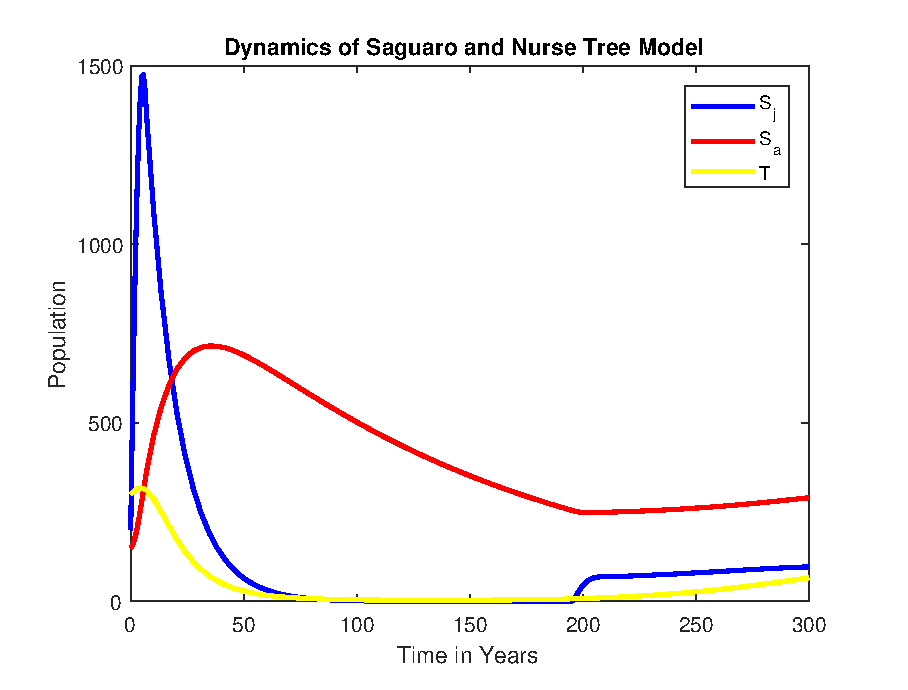
\includegraphics[scale = 0.7]{original_200_150_300.eps}
\caption{Dynamics of the original system with the baseline parameter values found in Table \ref{table:1} and the initial conditions $(S_j, S_a, T) = (200,150,300)$.}
\label{fig:original}
\end{center}
\end{figure}
The dynamics seen in Figure \ref{fig:original} show that when left to their natural life cycle, saguaros and nurse trees will coexist. The juvenile saguaro population increases to its carrying capacity and then begins to decline as the adult population increases, which is a result of the juveniles aging to $S_a$, or adulthood. Once the adult population declines to a certain level, there is now room for new juvenile saguaros, so then the juvenile population is able to increase. Because of competition, as the adult saguaro population increases, the tree population decreases, but begins to increase once the adult saguaro population has decreased to a certain level. Although the tree population appears to die out, it does not. The minimum value for $T$ in \ref{fig:original} is actually about $T = 3$. Eventually, all three populations are able to coexist. This is because the parameter values used in this simulation satisfy the conditions for coexistence and stability given in the analysis section. The simulation is calculated over a span of 400 years in order to account for the long lifespans of palo verdes and saguaros, which are about 100 and 175, respectively.\\

The dynamics of the tree and saguaro populations without buffelgrass are sensitive to changes in parameters $\phi$, $\rho$, $b$, and $r$. However, the only parameters from this list that could reasonable be changed in the real-world are $\phi$, the growth rate of trees, and $r$, the growth rate of juvenile saguaros. Each of these rates could be increased by planting new trees or saguaros.

\begin{figure}[H]
\hspace{-1.5 cm}
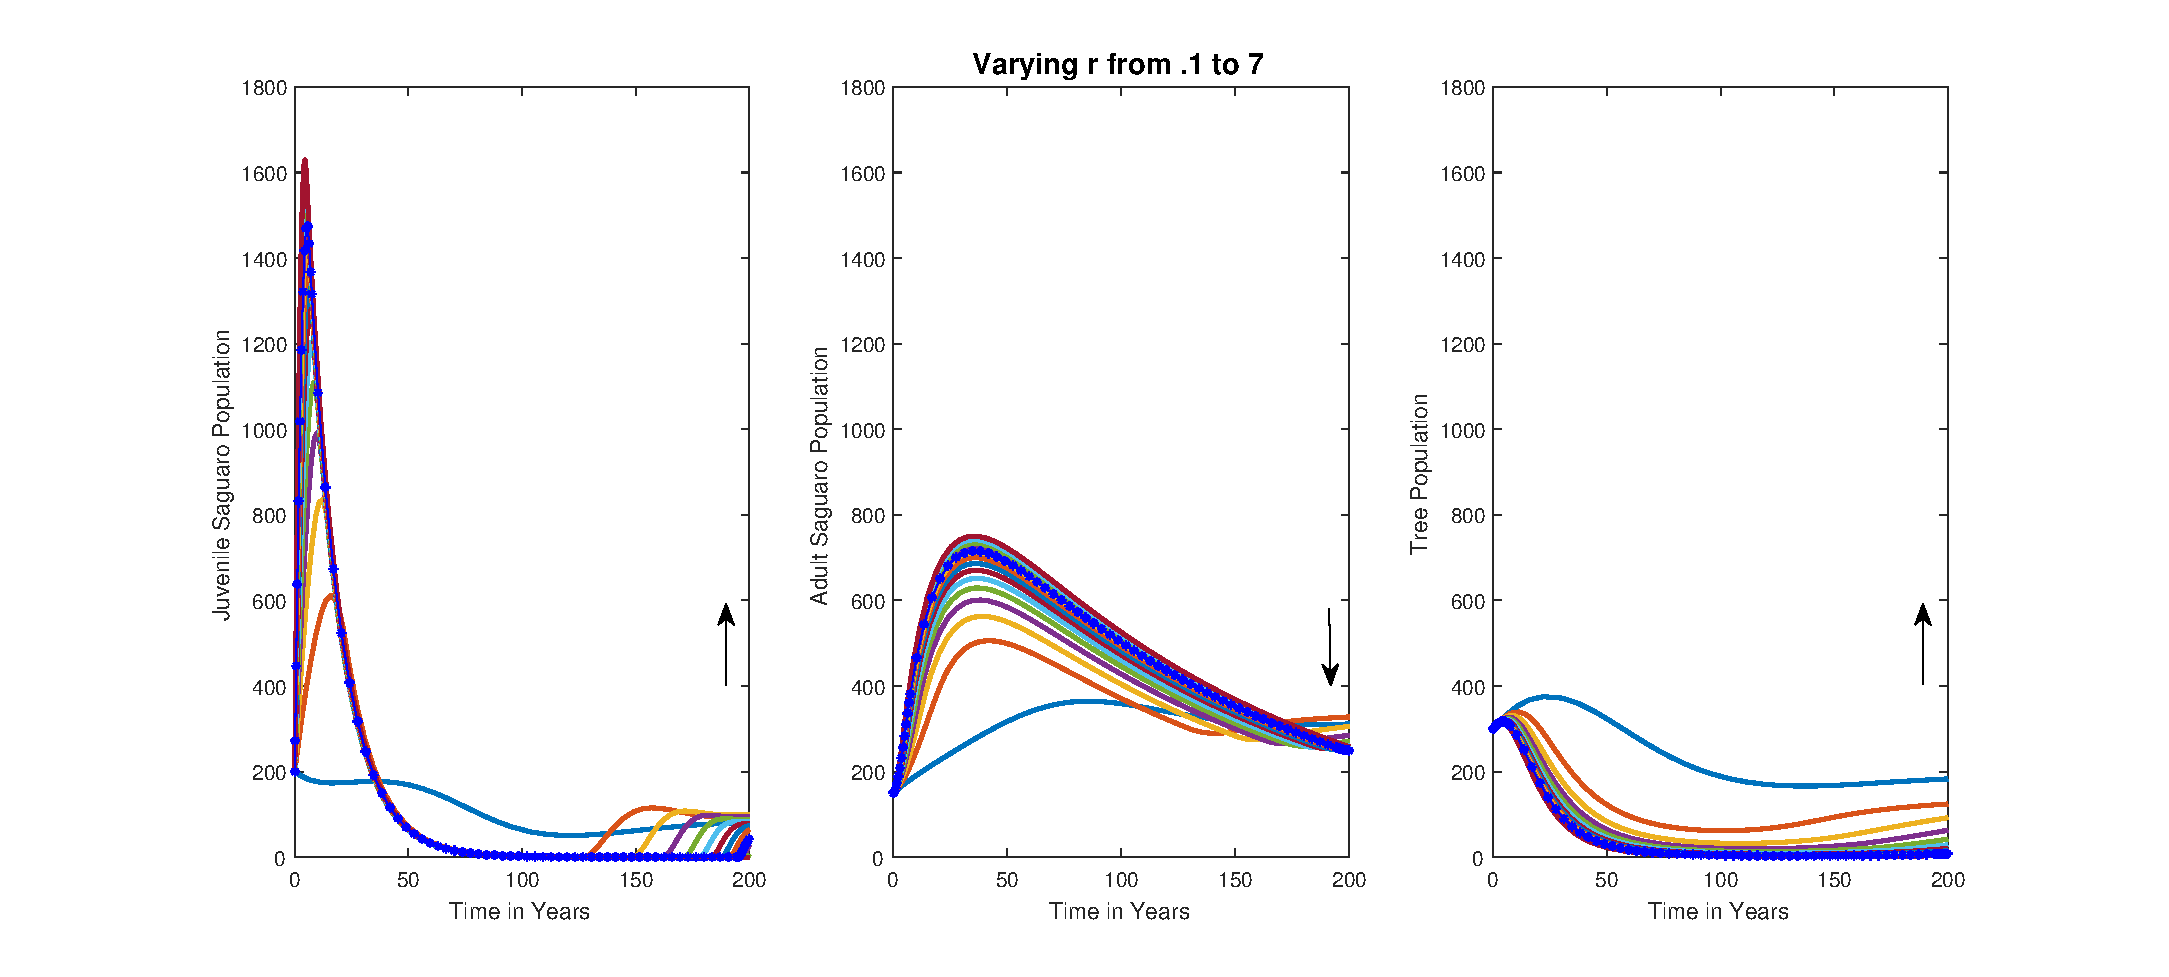
\includegraphics[scale = 0.5]{VaryRNoBuffel.eps}
\caption{The dotted blue line represents the baseline case for the parameters, given in Table \ref{table:1}. The arrows represent the direction that value of the equilibrium populations is changing.}
\label{fig:VaryR}
\end{figure}
In figure \ref{fig:VaryR}, as $r$ is increased, the final values for the populations $S_j$ and $S_a$ are not changed much. However, $S_j$ is slightly increased and $S_a$ is slightly decreased.This is because The final value for the population $T$ is slightly increased, because a decreased $S_a$ population decreases the competition faced by trees. It can be inferred that trying to increase the saguaro population by increasing the growth rate is not an effective strategy. However, varying $\phi$ has a greater effect.
\begin{figure}[H]
\hspace{-1.5 cm}
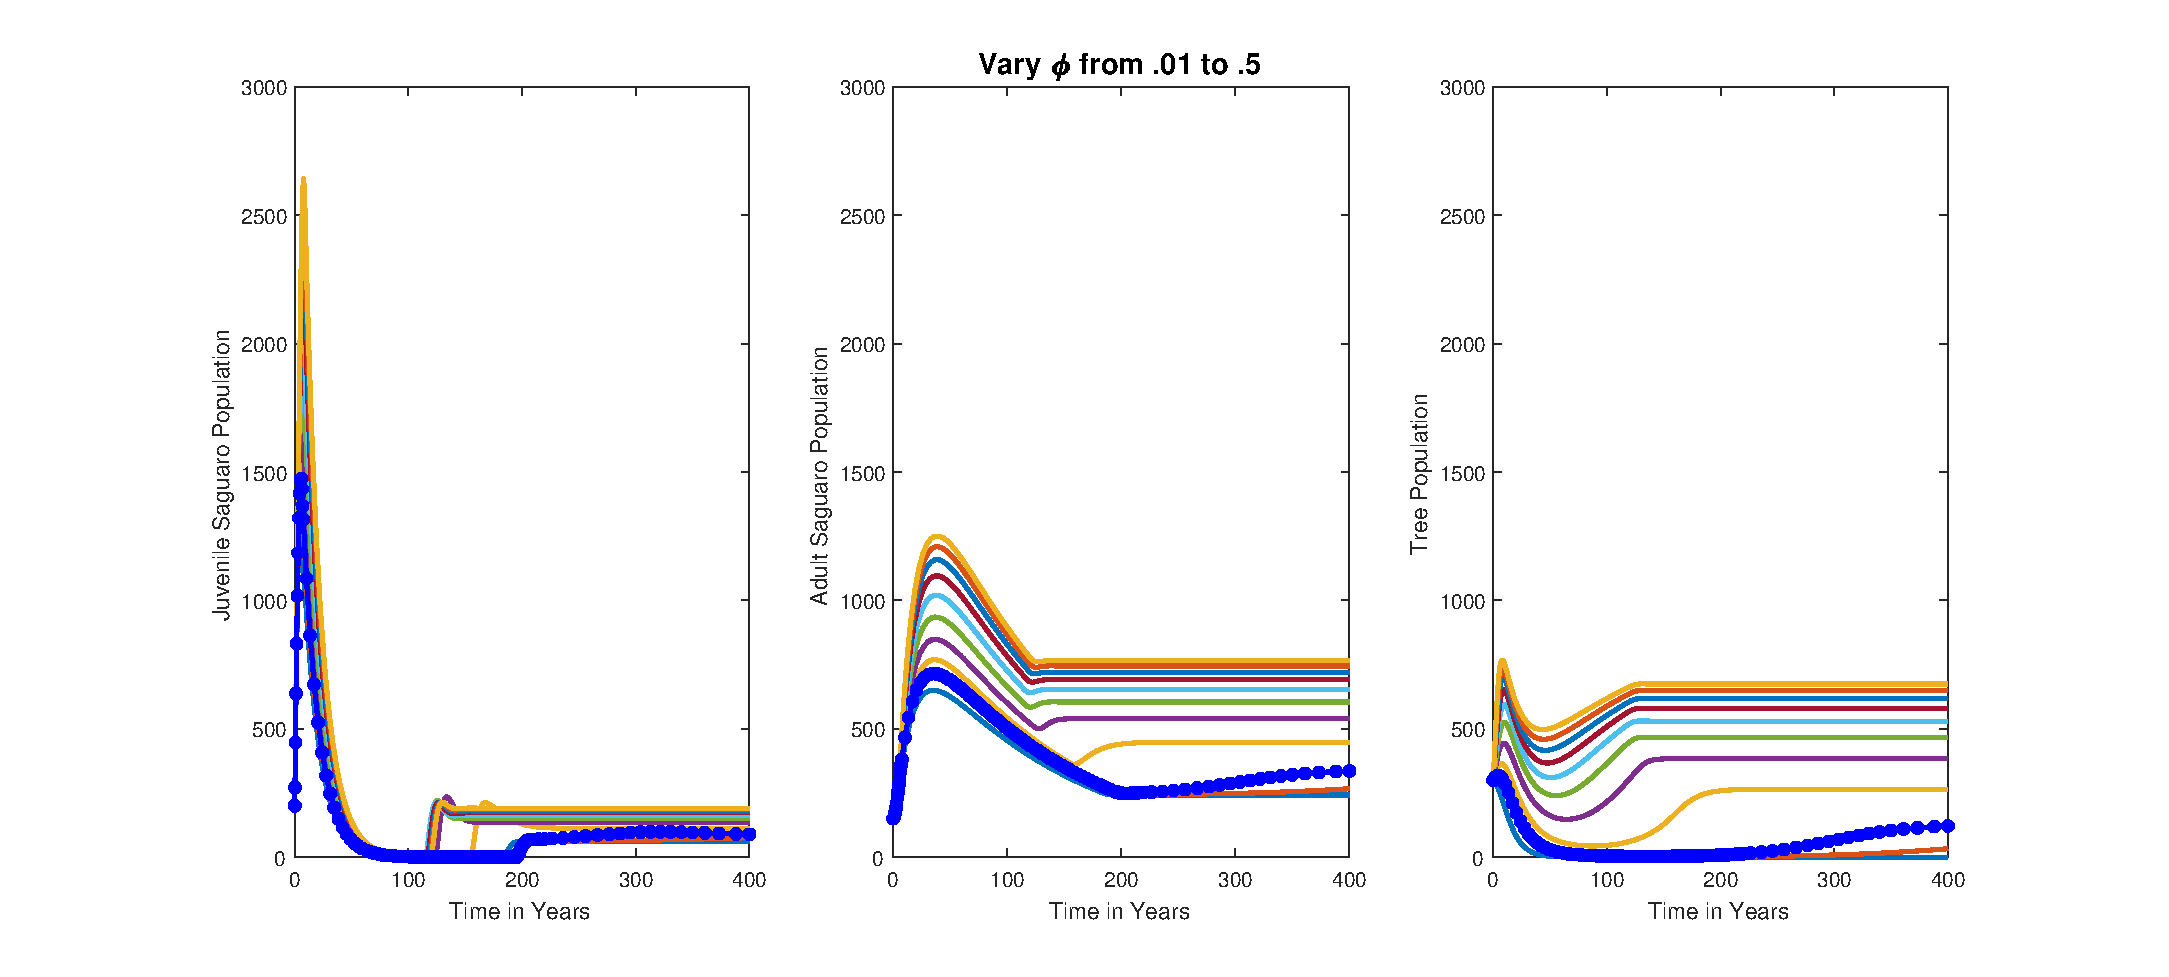
\includegraphics[scale = 0.5]{VaryPhiNoBuffel.eps}
\caption{The dotted blue line represents the baseline case for the parameters, given in Table \ref{table:1}. As $\phi$ is increased, the final values for the populations $S_j$, $S_a$, and $T$ also increase.}
\label{fig:VaryPhi}
\end{figure}
From Figure \ref{fig:VaryPhi}, it can be inferred that increasing $\phi$ in order to increase the saguaro population would be an effective strategy. This could be achieved through volunteers planting trees. Changing $\phi$ can also be thought of as having the same effect as changing $b$, because increasing $\phi$ increases the nurse tree population, which increases the term $bT$ . Since $bT$ increases the carrying capacity of juvenile saguaros, increasing this term results in a greater saguaro population.


\section{Population Dynamics after the Inclusion of Buffelgrass}
The effects of buffelgrass on the saguaro cactus and palo verde populations was incorporated in the $\theta$ terms in the model of section 2.3. These terms capture the death of saguaros by wildfire by taking an average of deaths per year instead of shocks to the population after a certain amount of time.
\begin{figure}[H]
\centering
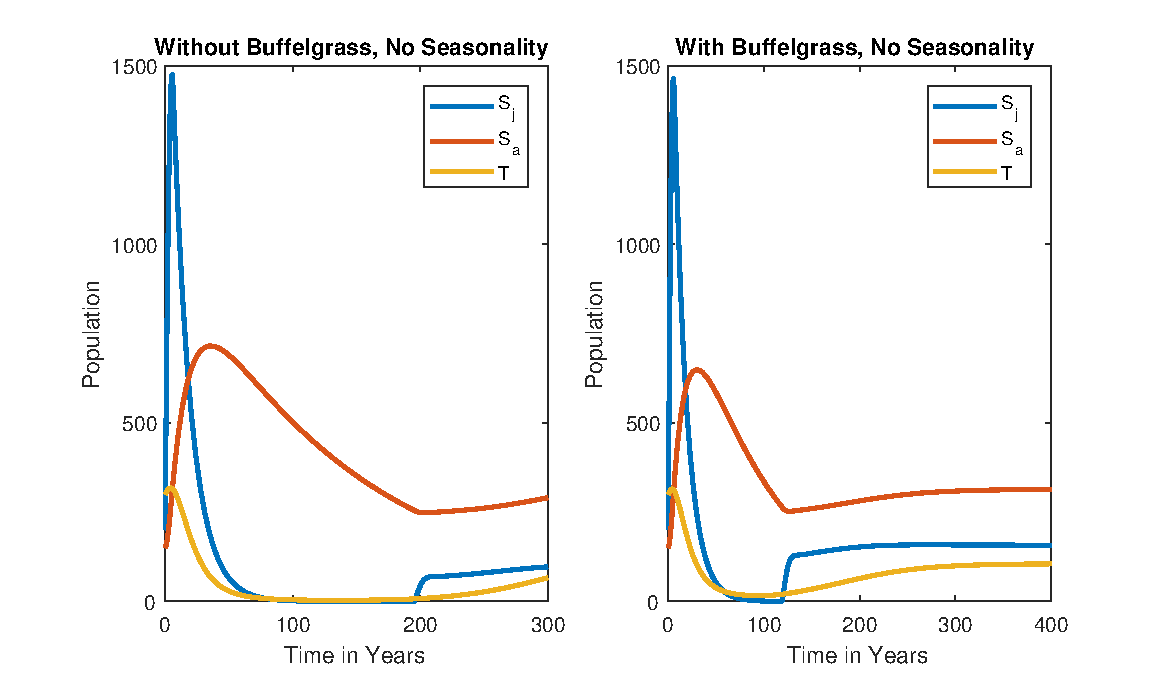
\includegraphics[scale = 0.7]{CompareWithBuffel.eps}
\caption{This figure compares the population dynamics of the saguaros and nurse trees with and without buffelgrass. }
\label{fig:includeBuffel}
\end{figure}
To show the dynamics of the populations, the buffelgrass populations were taken at equilibrium, $B=k_2 \left(1-\displaystyle\frac{\mu_b}{\omega}\right)=2857.14$, and our baseline paramater values. In figure \ref{fig:includeBuffel}, the buffelgrass population is not shown because the population is much larger than the other species, and because its dynamics are not affected by the other species. With the inclusion of buffelgrass, there is not a great change to the final population values, which can be due to the small values of $\theta$. However, the conditions for the coexistence equilibrium of the three species are met sooner. This is most likely because the saguaros are dying at a faster rate, creating more space for the tree population. \\

\subsection{Varying the Parameters Associated with Buffelgrass}
The following figures show the effects of increasing the $\theta$ values by increasing the frequency of wildfires on the populations.
\begin{figure}[H]
\hspace{-1.5 cm}
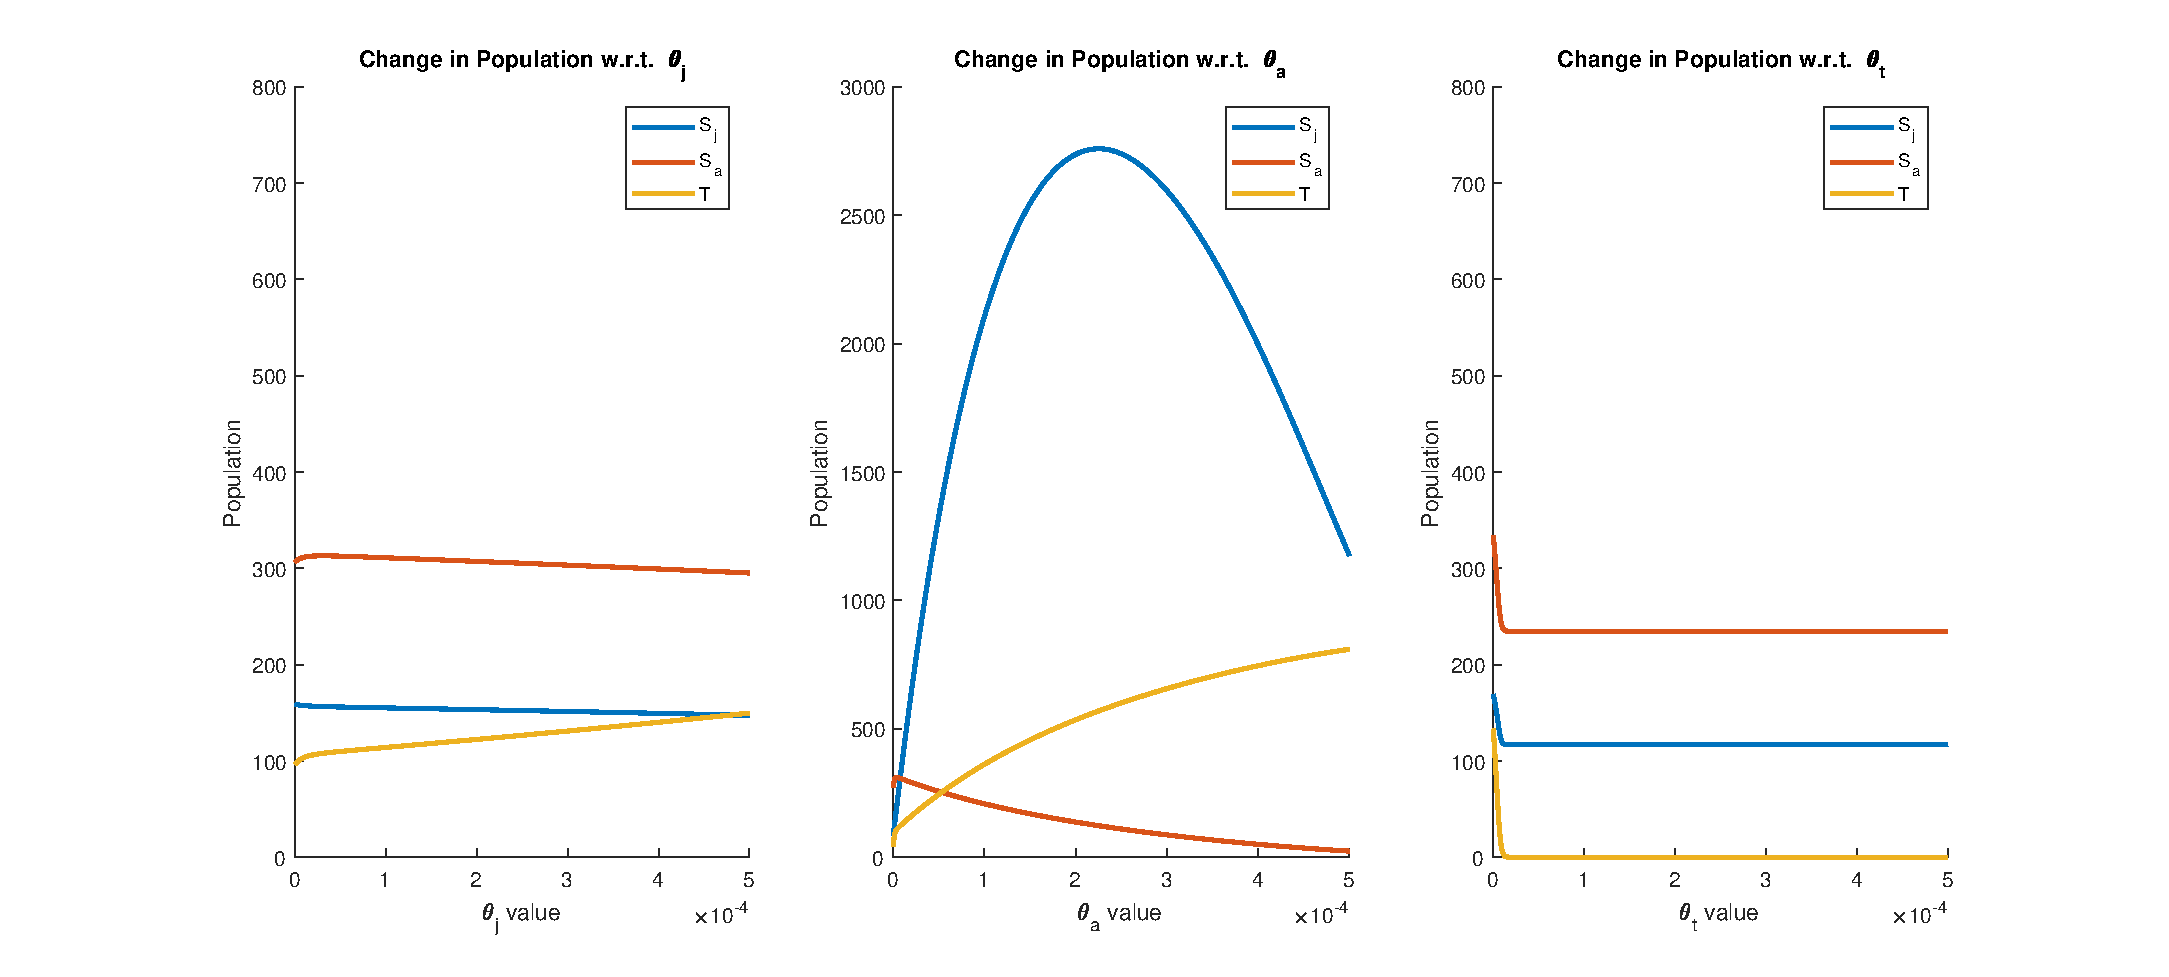
\includegraphics[scale = 0.5]{PopsVSThetas.eps}
\caption{This figure shows the effects of varying each $\theta$ on the saguaro and tree populations at time 400, when the populations have reached their equilibrium values. The y-axis gives the population values, and the x-axis gives the $\theta$ values.}
\label{fig:VaryThetas}
\end{figure}
From the first graph in Figure \ref{fig:VaryThetas}, it can be seen that varying $\theta_j$ does not result in much change in the equilibrium populations. Because the juvenile population is based on the adult population, increasing $\theta_j$ by itself does not greatly effect any of the populations. If it is greatly increased, $\theta_j$ will eventually cause the decline of the juvenile and adult saguaro populations and the increase in the palo verde population.\\ 

As the value of $\theta_a$ is increased, the adult saguaro populations approach extinction. However, the juvenile population increases with $\theta_a$ becomes too large. This is because juvenile saguaros compete with adult saguaros over space, so when adults die, there is more space available for juveniles. When there is no longer enough adult saguaro to produce juveniles, the juvenile population also begins to decline. The tree population increases because of the lack of competition. In reality, this would not occur because the increased frequency of fires would also affect the tree population.
As expected, in Figure \ref{fig:VaryThetas}, increasing the $\theta_T$ value does not greatly effect the adult and juvenile saguaro populations. However, increasing $\theta_T$ even by a small amount causes the palo verde population to become extinct. The slight decrease in the sagauro populations is because as the nurse tree population declines, fewer juveniles will be germinated and survive. This in turn causes a decrease in the adult population.\\

From Figure \ref{fig:VaryThetas}, it is reasonable to conclude that increasing the frequency of wildfires will drive both the saguaro and palo verde populations to extinction, if increased to a great enough frequency. Further evidence of this is in Figure \ref{fig:MoreFire}.\\
\begin{figure}[H]
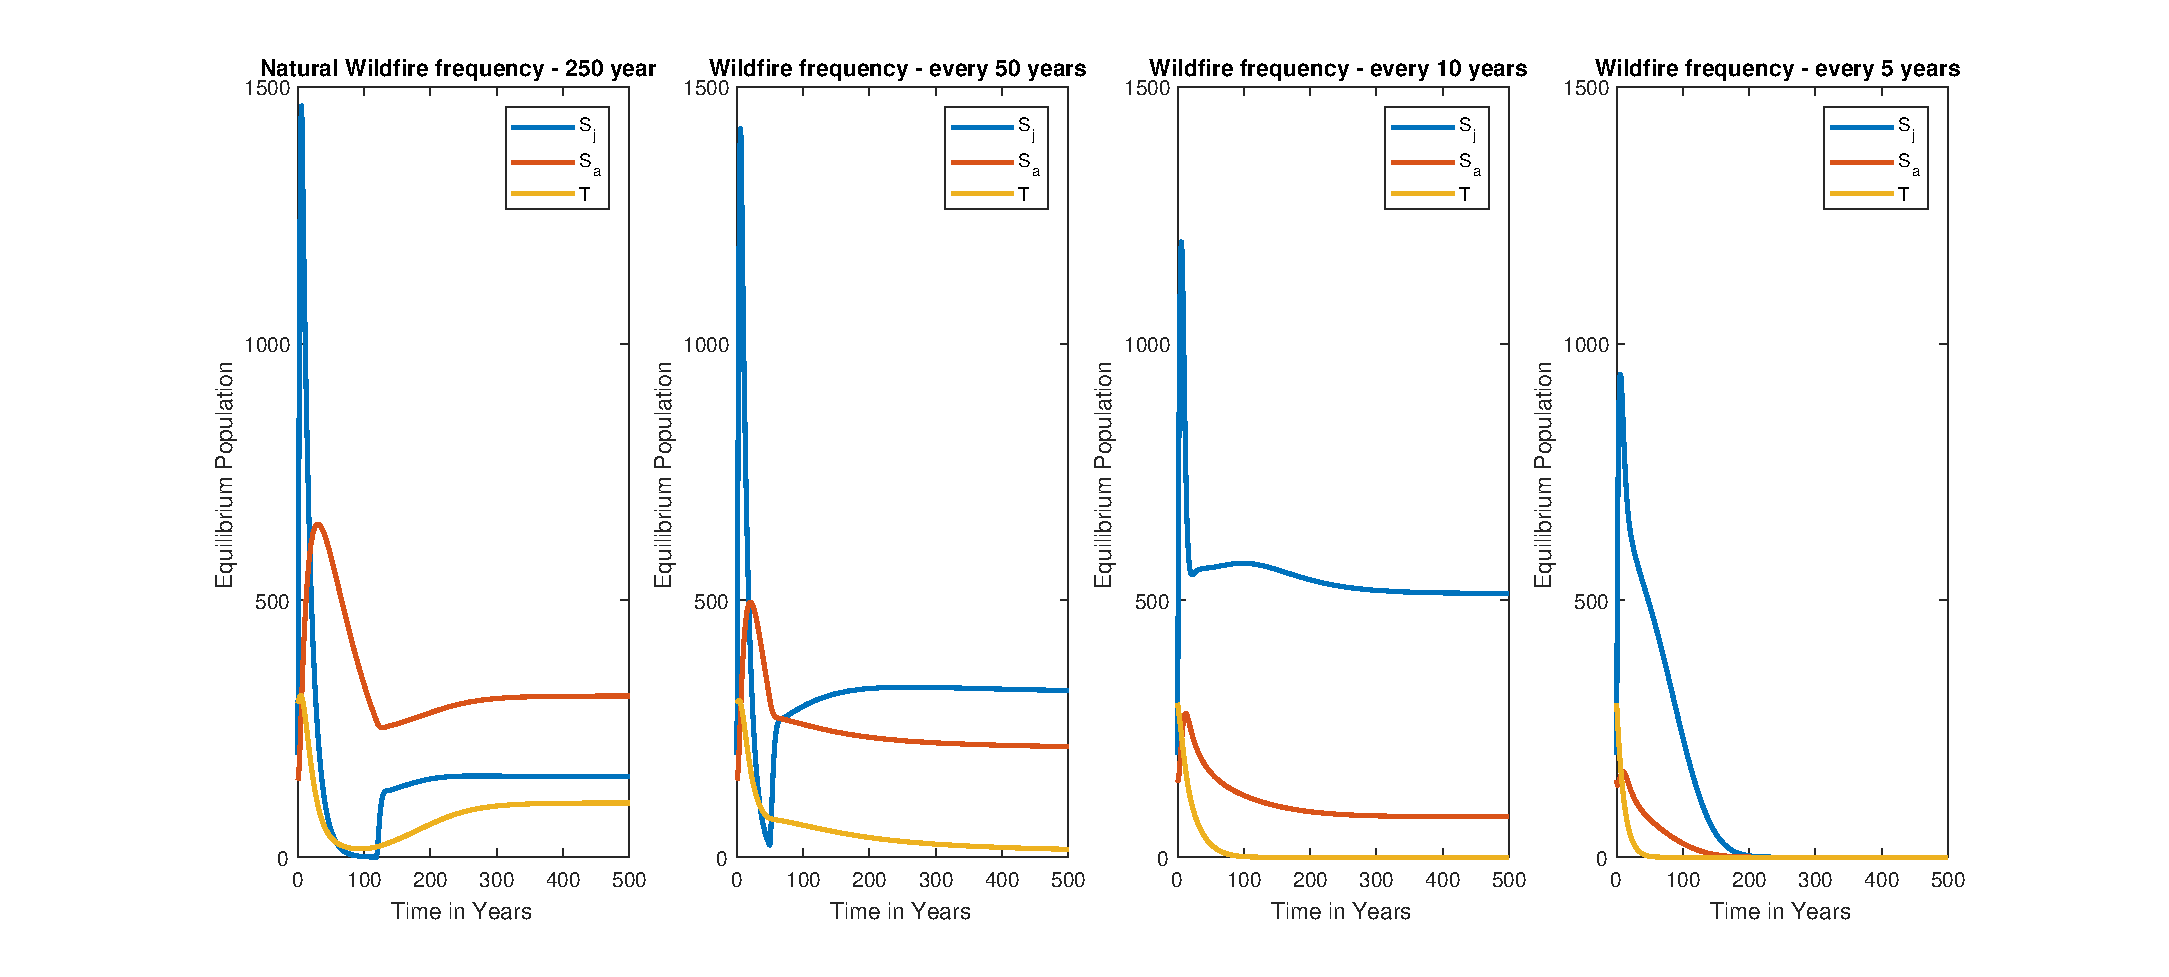
\includegraphics[scale = 0.4]{IncreasingWildfireFrequancy}
\caption{Here the wildfire frequency is increased and the resulting population dynamics of saguaros and nurse trees are shown.}
\label{fig:MoreFire}
\end{figure}
Since the current wildfire frequency in the Saguaro National Park could not be found, the true values of the $\theta$ terms are not known, and the value given in Table \ref{table:1} may not be accurate. Therefore, in order to answer the question as to whether buffelgrass will cause the extinction of the saguaro and nurse tree populations, different wildfire frequencies were tested with the model equations in Figure \ref{fig:MoreFire}. These results show that increasing wildfire frequency to every 10 years would result in the extinction of nurse trees, and increasing the frequency to every five years would eliminate saguaros. Since buffelgrass causes the increased spread of fires, we can assume that by reducing the amount of buffelgrass would allow the natural wildfire rate to hold.\\

The next step is to examine the effects of employing strategies to decrease the buffelgrass population. These strategies include reducing the growth rate, which could be done through chemical spraying, and increasing the harvesting term, by increasing the rate it takes to eliminate a patch of buffelgrass.


\begin{figure}[H]
\hspace{-2cm}
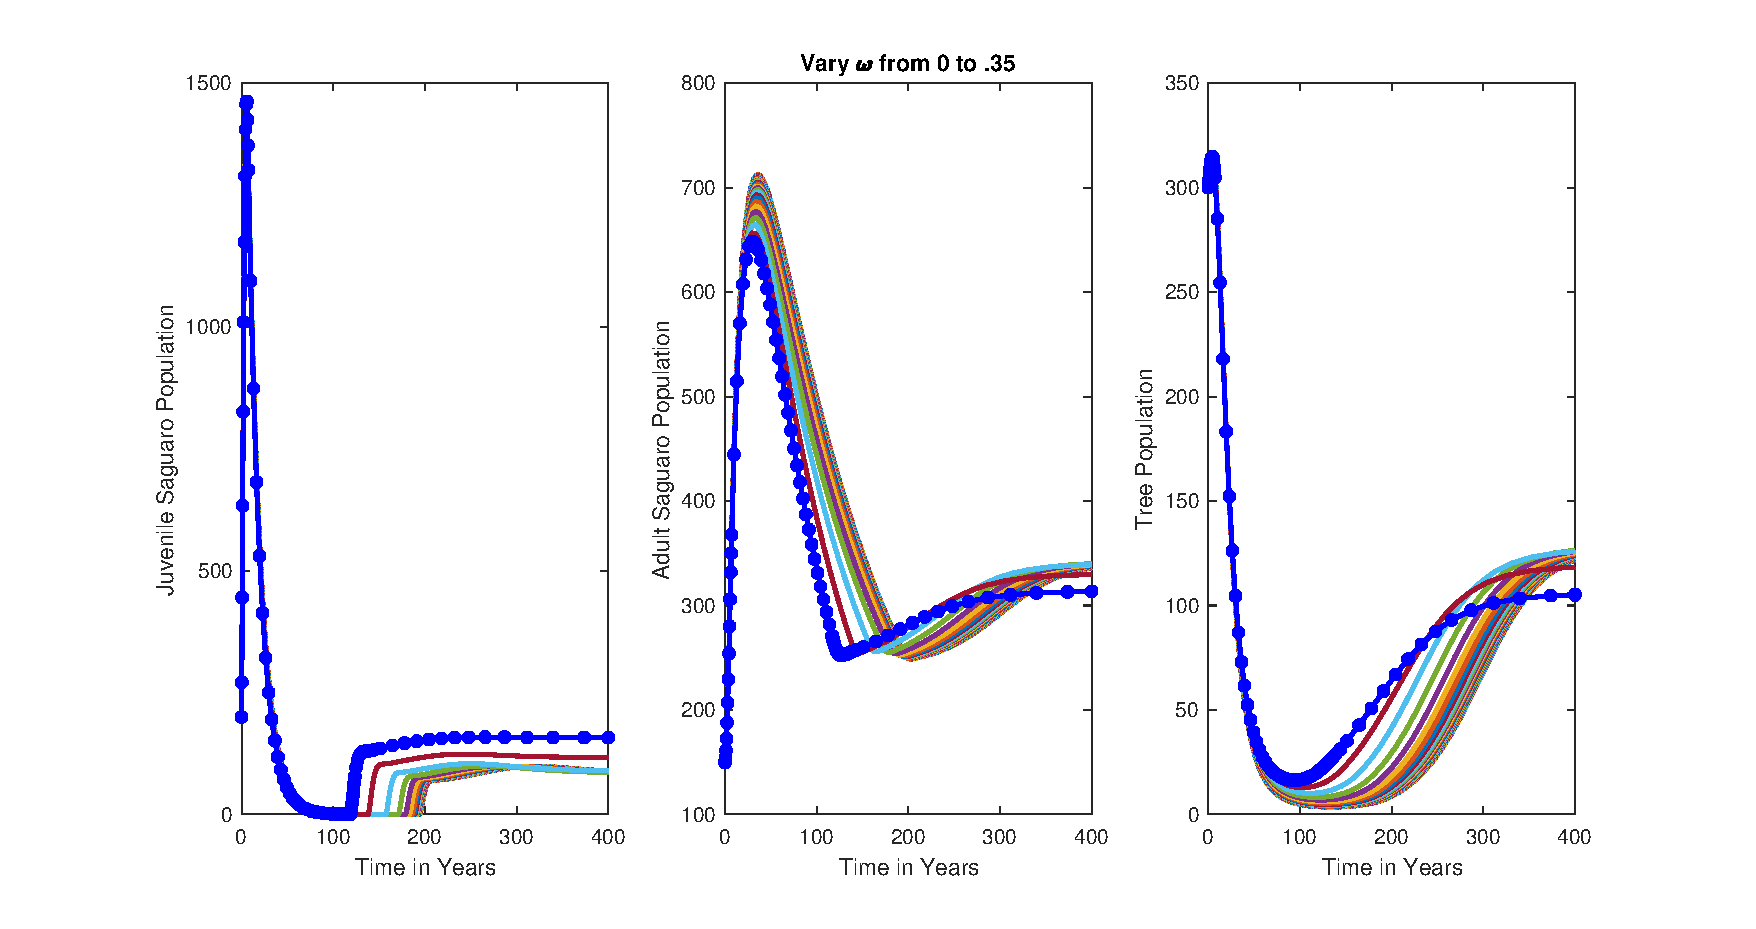
\includegraphics[scale = 0.55]{VaryOmegaWbuffel.eps}
\caption{This figure show the effects of decreasing $\omega$ from .35 to 0 on the population values of $S_j$, $S_a$, $T$. The blue dotted line is shows the dynamics with the baseline parameter value of $\omega = .35$.}
\label{fig:VaryOmega}
\end{figure}
Figure \ref{fig:VaryOmega} shows the changes in the juvenile and adult saguaro and tree populations from decreasing $\omega$. These changes include greater resulting populations for adult saguaros and trees. However, the resulting juvenile population is smaller, which is because more saguaros are able to age into adulthood, which decreases the available space for new juveniles. Although the equilibrium tree population increases, it takes longer for the tree population to grow back after the initial decrease due to competition with the growing adult saguaro population. This is because the peak value for the adult population increases with the decrease of $\omega$ and slows the growth of trees through competition. 

\begin{figure}[H]
\hspace{-1.5 cm}
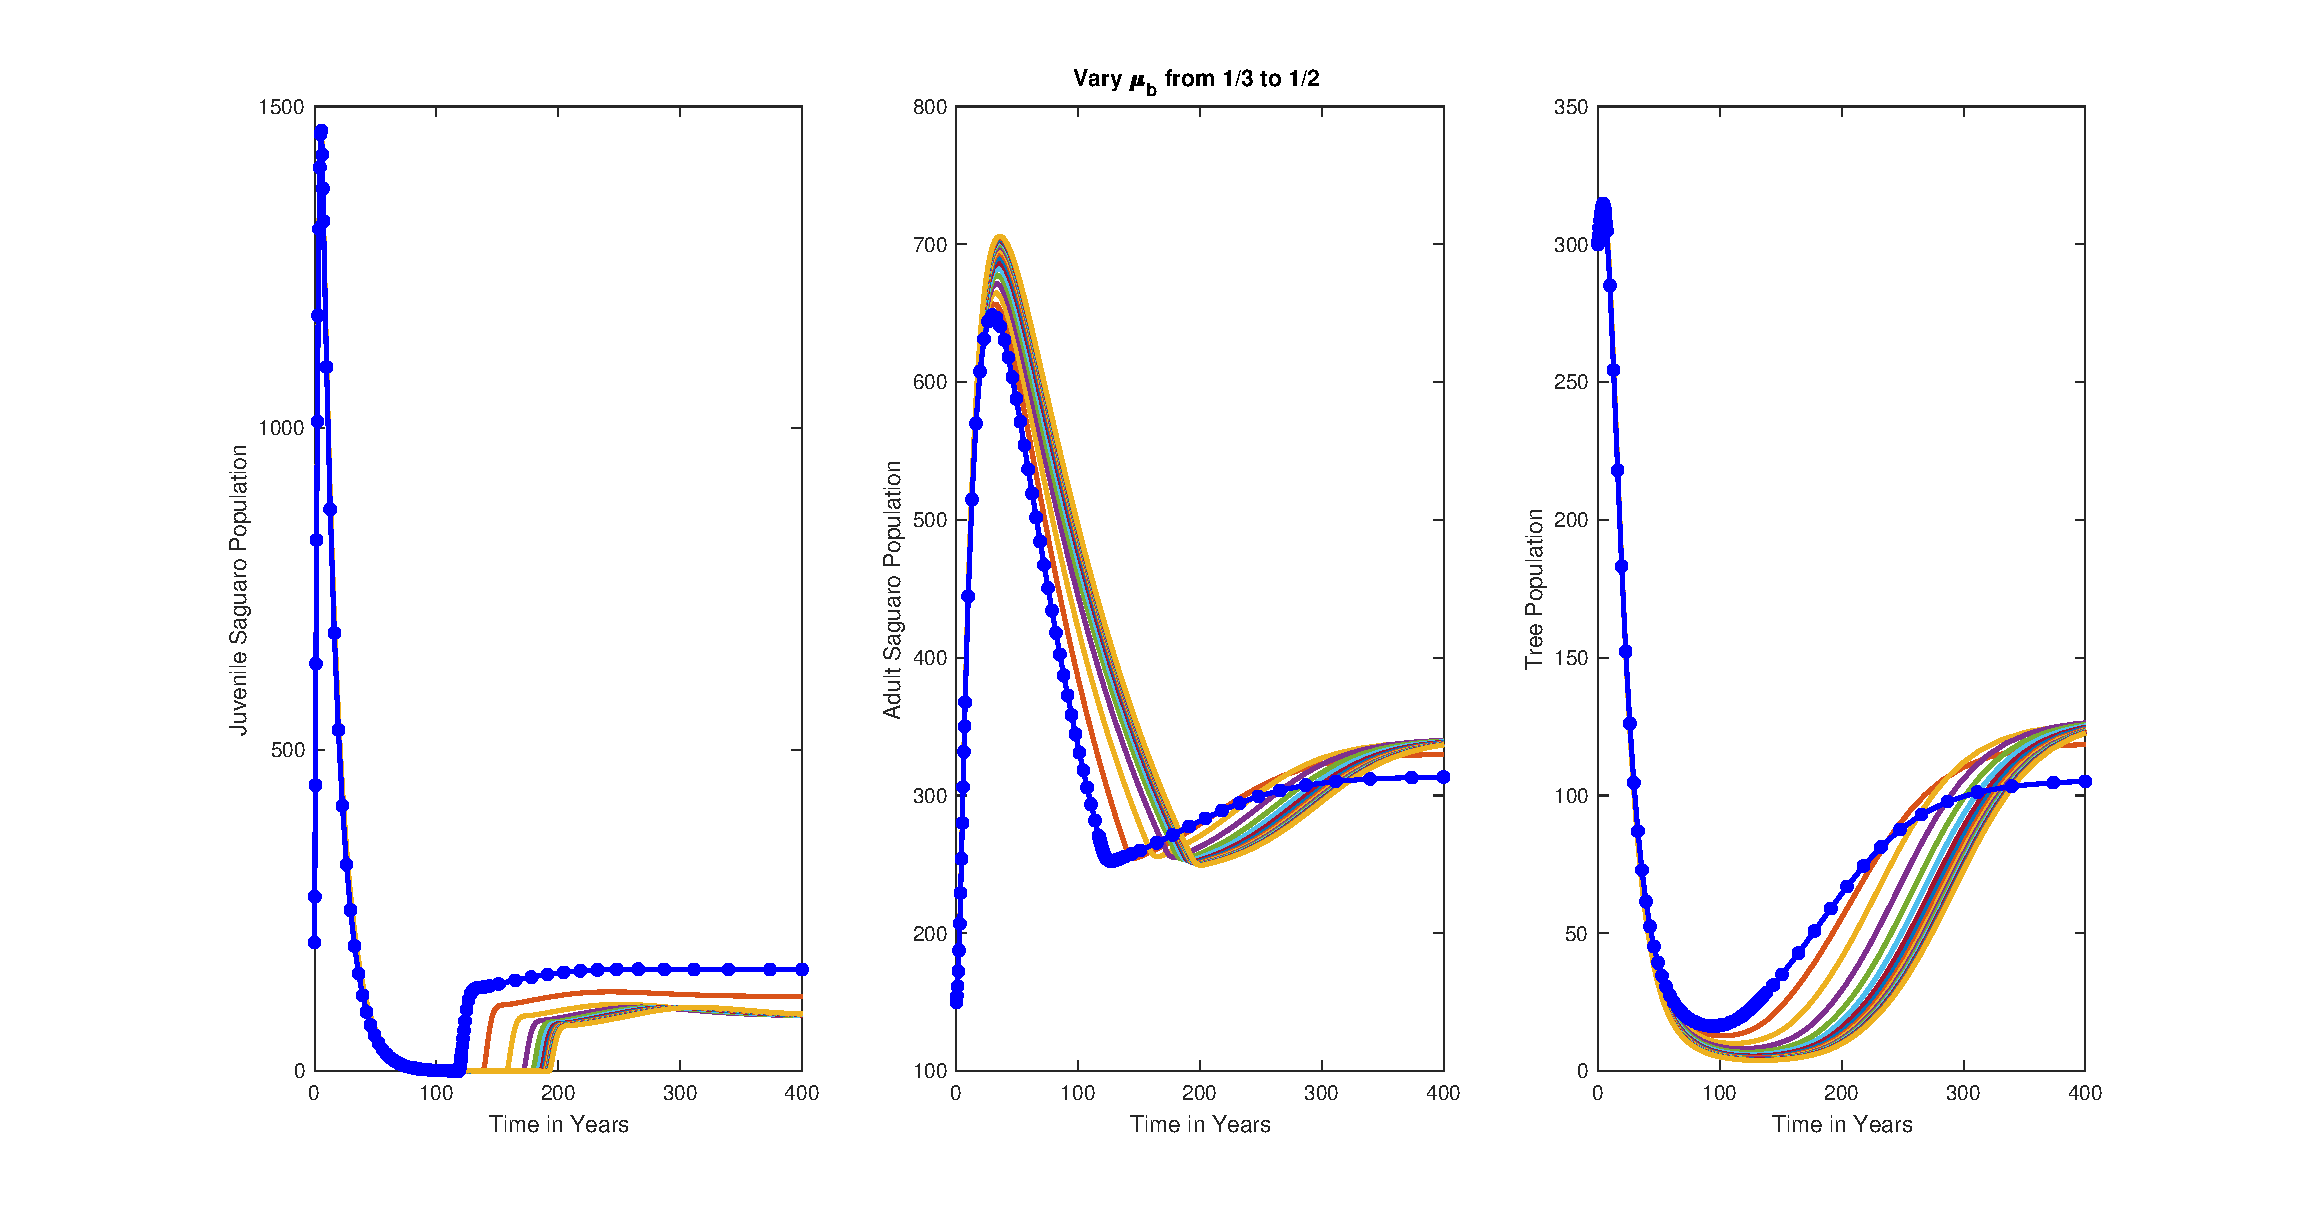
\includegraphics[scale = 0.5]{VaryMubWbuffel.eps}
\caption{This figure show the effects of increasing $\mu_b$ from $\frac{1}{3}$ to $\frac{1}{2}$ on the saguaro ant tree population values. The dotted, blue line represents the dynamics with the baseline parameters, $\mu_b = \frac{1}{3}$}
\label{fig:VaryMub}
\end{figure}

The results of Figure \ref{fig:VaryMub} are similar to those of Figure \ref{fig:VaryOmega}. In Figure \ref{fig:VaryMub}, it can be seen that increasing the harvesting rate can increase the adult saguaro and nurse tree populations, while decreasing the juvenile population at the final time in the simulation, because more saguaros are able to age into adulthood and therefore take up space that would otherwise be available for juveniles.\\

Therefore, from Figures \ref{fig:VaryOmega} and \ref{fig:VaryMub}, it can be inferred that taking measures to reduce the growth rate and increase the harvesting rate of buffelgrass would result in larger adult saguaro and tree populations.
\subsection{Numerical Simulations of Coexistence Conditions and Stability}
Using the parameter values given in Table \ref{table:1}, the coexistence of the saguaro and nurse tree population can be verified with and without the inclusion of buffelgrass.
\subsubsection{Coexistence without Buffelgrass}
In order to verify that saguaros and nurse trees coexist without buffelgrass, it is necessary to prove that the conditions described in section 3.2.4 hold true for the estimated parameter values. The conditions for having at least one positive root are as follows:
\begin{subequations}
\begin{equation}
\displaystyle\frac{\phi}{\rho}>\displaystyle\frac{k_1}{1+E}\left(1-\displaystyle\frac{1}{R_{d1}}\right)
\end{equation}
\begin{equation}
R_{d2} > 1
\end{equation}
\end{subequations}
with the parameter values given in Table \ref{table:1}, these conditions are satisfied.
That is, since these conditions are shown to be true, the model will have at least one coexistence equilibrium. Furthermore, once the possible equilibria values are found, the condition
\begin{equation}\label{eq:exist}
S_a^*<\displaystyle\frac{\phi}{\rho}
\end{equation}
must be satisfied for each in order for two coexistence equilibria to exist.\\

The equilibria population values of the trees and juvenile saguaros depend on the quadratic equation for the value of $S_a$. Solving this quadratic gives two possible equilibrium populations for the adult saguaro population, $S_{a1} = 341.225$ and $S_{a2} = 3.97549*10^8$. Since only the equilibrium point, $S_a = 341.225$ satisfies Equation \ref{eq:exist}, there is only one coexistence equilibrium. For the existing equilibrium population of $S_a$, the other population values are $S_j = 85.3079$ and $T = 127.726$.\\

The stability of the existing coexistence equilibrium can be proven by inputing the baseline parameters from Table \ref{table:1} and the equilibrium population values into the Jacobian of the model equations from Equation \ref{eq:noBuffelJacobian} in the appendix.\\

The eigenvalues of the resulting matrix are 
$$\vec{v} = \begin{pmatrix}
-0.287472 + 0.201232i\\
-0.287472 - 0.201232i\\
-0.0294237 + 0.i
\end{pmatrix}$$ 
Since the real part of each eigenvalue is negative, the equilibrium point is stable. Because the eigenvalues are imaginary, there is a possibility for oscillations or spiraling behavior to occur. However, with the current parameter values given in Table \ref{table:1}, values for the tree population and total saguaro population never drop to zero or below, meaning that there are no oscillations or spiraling behavior.
\subsubsection{Coexistence with Buffelgrass}
To verify the coexistence of the saguaro populations, nurse trees, and buffelgrass we need to check the conditions mentioned in section 4.2.1.4 hold true for the estimated parameter values. The conditions for the existence of two roots are the following.
\begin{equation*}
\displaystyle\frac{\tilde{\phi}}{\rho}>\displaystyle\frac{k_1}{1+\tilde{E}}\left(1-\displaystyle\frac{1}{R_{d3}}\right)
\end{equation*}
\begin{equation*}
R_{d4} > 1
\end{equation*}

With the baseline parameters values given in Table \ref{table:1}, and the new parameters for the buffelgrass model from the Appendix A section 2, these conditions are satisfied.
Since these conditions are shown two be true, the model will have two possible coexistence equilibria. The equilibria population values of the trees, juvenile saguaros, and buffelgrass depend on the quadratic equation for the value of $S_a^*$, and existence depends on the equation
\begin{equation}\label{eq:existb}
S_a^*<\displaystyle\frac{\tilde{\phi}}{\rho}
\end{equation}
Solving the quadratic for $S_a^*$ gives two possible equilibrium populations for the adult saguaro population, $S_{a1} = 313.478$ and $S_{a2} = \num{5.95358e9}$. However, only one of these values satisfies Equation \ref{eq:existb}, $S_a = 341.225$. For the existing equilibrium population of $S_a$, the other population values are $S_j = 157.588$, $T = 105.202$, and $B = 2857.14$.\\

The stability of the existing coexistence equilibrium can be proven by inputing the baseline parameters from Table \ref{table:1}, the new parameters for buffelgrass model from the Appendix A section 2, and the equilibrium population values into the Jacobian of the model equations from Equation \ref{eq:noBuffelJacobian} in the appendix.

The eigenvalues of this matrix are $$\vec{v} = \begin{pmatrix}
-0.290433 + 0.201589i\\
-0.290433 - 0.201589i\\
-0.0166667 + 0i\\
-0.0162684 + 0i\\
\end{pmatrix}$$ 
Since the real part of each eigenvalue is negative, the equilibrium point is stable. Because the eigenvalues are imaginary, there is a possibility for oscillations or spiraling behavior to occur. However, with the current parameter values given in Table \ref{table:1}, values for the tree population and total saguaro population never drop to zero or below, meaning that there are no oscillations or spiraling behavior.
\section{Sensitivity Analysis}
The type of sensitivity analysis used for the model is a local sensitivity analysis, which quantifies the effects of slightly perturbing the value of a critical parameter on a quantity on interest. In this case the value of the critical parameter is changed by one percent change and the quantities of interest are the equilibrium populations. However, these results are only valid for a small region around the baseline solution. When looking at the results in Tables \ref{table:NormalSensitivity} and \ref{table:BuffelSensitivity}, it is important to note that the sign of each sensitivity index gives the direction of the change in the quantity of interest, and the value gives the magnitude of the change in percentage. \cite{sensitivitySource}.
\subsection{Sensitivity Analysis of Critical Parameters without Buffelgrass}
In this section sensitivity analysis is going to be performed on critical parameters of the basic model without buffelgrass. The parameters being analyzed the rate that seeds are germinated and survive to one year, $r$, the average number of juveniles that survive under a nurse tree per tree, $b$, and the logistic growth term for palo verde population, $\phi$.
\small{
\begin{center}
\hspace{-.8cm}
\begin{tabular}{|c|c|c|c|c|}\hline
{Sensitivity Analysis}
& $r$ & $b$ & $\phi$\\
\hline
$S_j$ &  0.0013& 0.1006 & 0.6534\\
\hline
$S_a$ & 0.0013 & 0.1006 & 0.6534\\
\hline
$T$ & -0.0084 & -0.6534 & 2.2520\\
\hline
\end{tabular}
\end{center}
}
In Table \ref{table:NormalSensitivity} it can be seen that for all critical parameters, $S_a$ and $S_j$ have the same sensitivity index with respect to these parameters. this is because any change in the juvenile population will effect how many saguaros will reach maturity, or become adults. Furthermore, any change in the adult population will effect how many new juvenile saguaros are produced. Therefore affecting one population will affect the other by an equal amount at equilibrium. Furthermore, Table \ref{table:NormalSensitivity} shows that increasing $r$, the germination rate of juvenile saguaros, by 1\% will only slightly affect the saguaro and nurse tree populations, increasing the saguaros by .001\%and decreasing the nurse trees by .0084\% due to competition with the increased adult saguaro population. The parameter $b$, has a greater effect on the equilibrium populations than $r$ and increases the saguaro populations by .1006\% when increased by 1\%. This is because the carrying capacity of juveniles is increased by increasing $b$, which increases $bT$, resulting in more juveniles and thus more adults. The tree population is decreased by .6534\% due to increased competition. The parameter $\phi$ had the greatest effect on all of the populations. Increasing $\phi$ by 1\% allows for the tree population to grow by 2.2520\%. This increase allows the juvenile population to grow through an increased carrying capacity and thus allows the adult population to grow. Therefore, increasing $\phi$ is not only the most efficient way to increase saguaro population in the absence of buffelgrass, but also promotes the growth of the tree population. 

\subsection{Sensitivity Analysis of Critical Parameters Dealing with Buffelgrass}
One of the goals of this study is to see the impact of wildfires and buffelgrass on the saguaro and nurse trees populations. Therefore, a local sensitivity analysis is performed on the $\theta$s, $\mu_b$ and $\omega$ parameters. This analysis will support the results of the simulations above.
\begin{table}[H]
\begin{tabular}{|>{\centering\arraybackslash}m{1.3cm}|>{\centering\arraybackslash}m{1.95cm}|>{\centering\arraybackslash}m{1.2cm}|>{\centering\arraybackslash}m{1.2cm}|>{\centering\arraybackslash}m{1.2cm}|>{\centering\arraybackslash}m{1.2cm}|}
\hline
{Sensitivity Analysis}
& $\theta_j$ & $\theta_a$ & $\theta_T$ & $\mu_b$ & $\omega$ \\
\hline
$S_j$ &  \num{-3.9182e-04} & 0.4916 & -0.0753 & -8.3189 & 8.3232 \\
\hline
$S_a$ & \num{-3.9184e-04} & -0.0111 & -0.0753 & 1.7351
 & -1.7354 \\
\hline
$T$ & 0.0028 & 0.0803 & -0.2980 & 4.2973 & -4.2973\\
\hline
$B$ & N/A & N/A & N/A & -20 & 20\\
\hline
\end{tabular}
\caption{The table above gives the sensitivity index of the population values of $S_j$, $S_a$, $T$, and $B$ after 400 years when changing the parameter values by 1\% from their baseline value given in Table \ref{table:1}.}
\label{table:BuffelSensitivity}
\end{table}
For the analysis in Table \ref{table:BuffelSensitivity}, the populations were used at their equilibria values, that is $S_j= 157.588$, $S_a=313.478$, $T=105.202$, and $B=2857.14$. This analysis shows that when increasing $\theta_j$ by 1\% the saguaro population decreases by 3.9\%, and th tree population increases by 0.0028\% since there is less competition with adult saguaros. The increase of $\theta_a$, will directly decrease adult saguaro population by 0.1\% but will increase the juvenile saguaro population by 0.49\% since it creates more available space for their establishment. The increase of $\theta_a$ will also positively affect the tree population by increasing it by 0.08\%, since the death of adult saguaros decreases the competition between them and the trees. On the other side, the increase of $\theta_T$, will decrease the saguaro population by 0.07\% and decrease the tree population by 0.29\%. Furthermore, it can be seen that the saguaro, nurse tree, and buffelgrass populations are most sensitive to changes in $\mu_b$ and $\omega$. The increase of $\mu_b$ would decrease the buffelgrass and juvenile saguaro populations by 20\% and8.32\% respectively, and increase the adult saguaros and trees by 1.73\% and 4.29\% respectively. The biological explanation to this change is that more juvenile saguaros are becoming adults, and this leaves less available space for new juvenile establishments. Finally, the increase of $\omega$ will increase the buffelgrass and juvenile saguaros populations by 20\% and 8.32\% respectively, but decrease the adult saguaros and trees by 1.73\% and 4.29\% respectively. Since there is more buffelgrass, there is less juvenile saguaros becoming adults and staying in the juvenile class, which declines the growth rate of the adult and tree population. Therefore, from these result, the most efficient way to protect the saguaro and nurse tree populations would be to reduce the buffelgrass population by either decreasing $\omega$ or increasing $\mu_b$. 
\section{Adding Seasonality without Buffelgrass}
To incorporate the seasonal dynamics of the saguaro populations, the reproduction rate is changed, $r$ and the death terms for the saguaro populations $\mu_j$ and $\mu_a$ to be functions of time. In the literature, it was found that saguaros only reproduce for a two month period of the year from May to June, June to July, or July to August. The particular two month period depends on location \cite{SaguaroBook}. \\
For the reproduction rate, a sinusoidal function is created to force the expected behavior of the growth rate.
\begin{equation}\label{eq:cosBirth}
r_{new}(t) = (2\cdot r_{avg})\cdot \cos^{14}\left(3t+\frac{\pi}{2}\right)
\end{equation}
In the equation \ref{eq:cosBirth}, $3t+\frac{\pi}{6}$ is used to center the function over the middle of the year so that births only occur between May and August. This is also the reason $\cos14^{th}$ is used, to force the rate to be centered over the middle of the year. The amplitude is the average growth rate, or $r_{avg}$.
\begin{figure}[H]
\centering
\includegraphics[scale = 0.7]{seasonalBirth.eps}
\end{figure}
For the death rate of the adult and juvenile saguaros, respectively, we have,
\begin{equation*}
\mu_{\text{a new}} = \mu_{\text{a avg}}\cdot \cos^{14}(3.15t) + \mu_{\text{a natural}}
\end{equation*}
and
\begin{equation*}
\mu_{\text{j new}} = \mu_{\text{j avg}}\cdot \cos^{14}(3.15t) + \mu_{\text{j avg}}
\end{equation*}
Similarly to the growth rate equation, the $\cos^{14}(3.15t)$ term is used to force the death rate to increase in the winter months, when saguaros in both age groups are susceptible to freezing temperatures. For the adults, the amplitude is the average death rate due to freezing and the cosine function is added to the rate that saguaros reach their natural lifespan. For the juvenile saguaros, the minimum of the function is the average death rate, which doubles in winter months.
\begin{figure}[H]
\centering
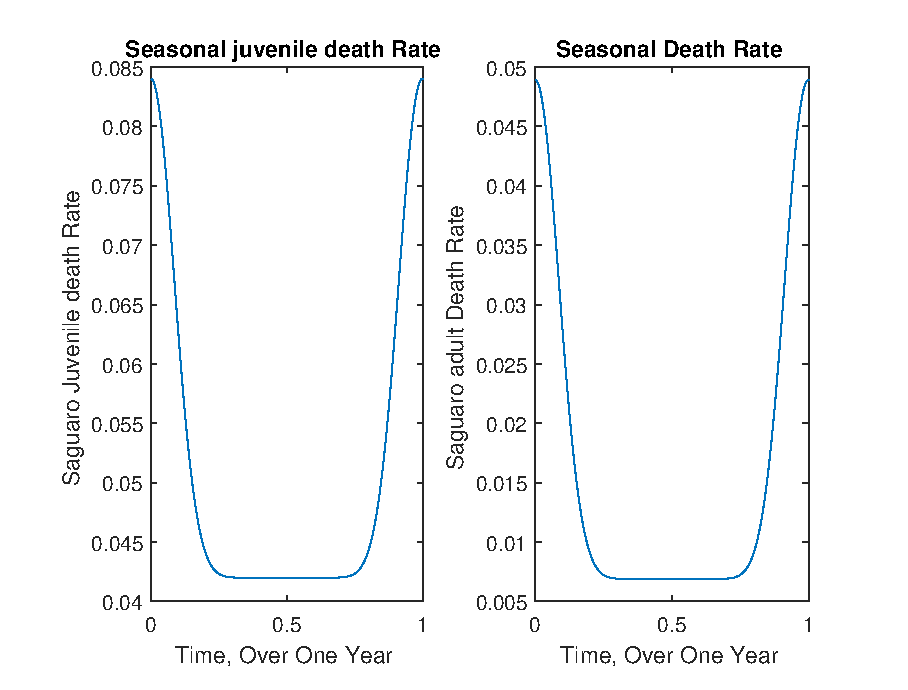
\includegraphics[scale=0.7]{SeasonalDeath.eps}
\end{figure}

The resulting changes in the model can seen in Figure \ref{fig:WithAndWithoutSeasonality}.
\begin{figure}[H]
\centering
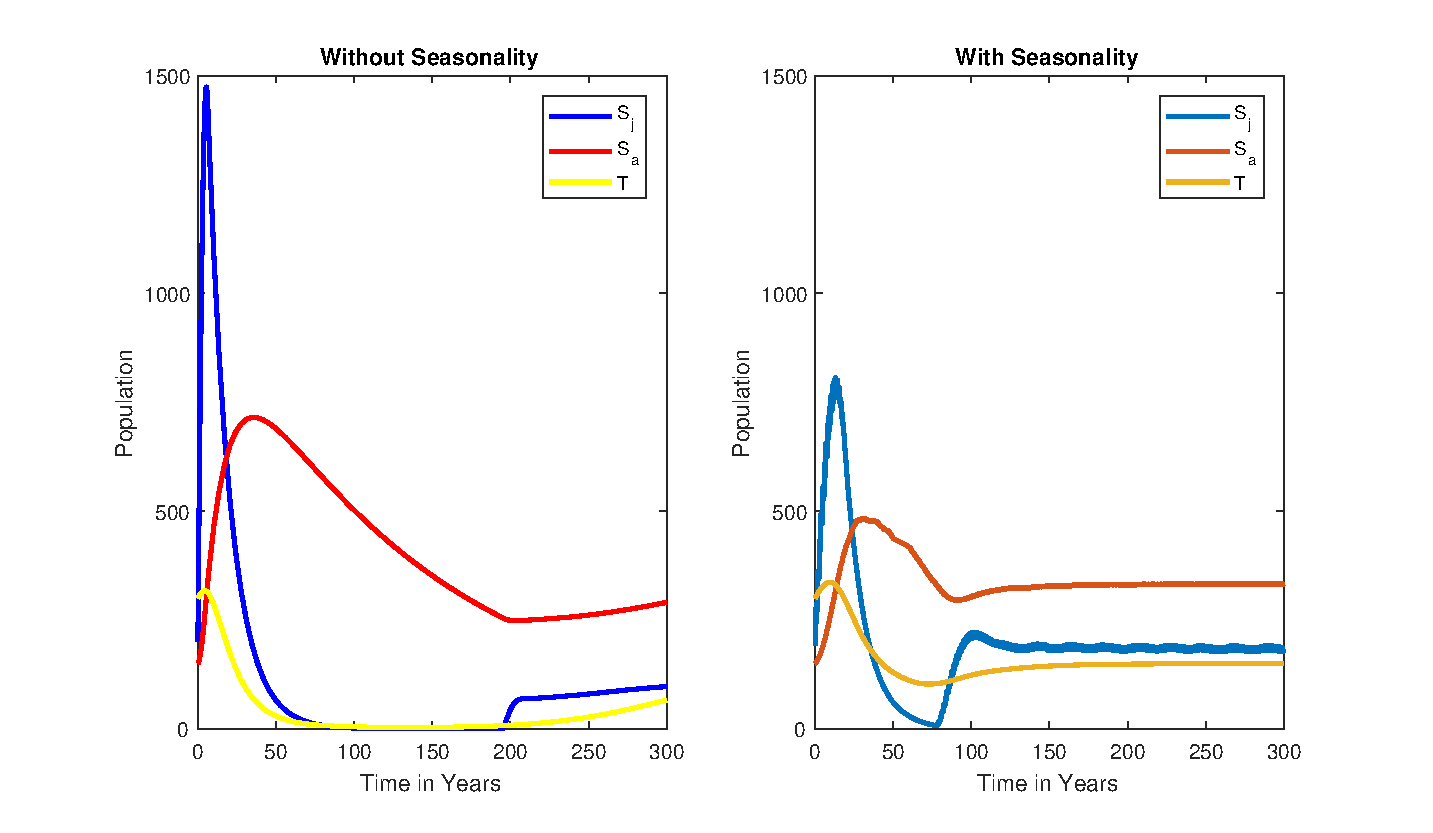
\includegraphics[scale = 0.45]{withAndWithoutSeasonality.eps}
\caption{This figure shows the difference in the systems with and without seasonality and uses the baseline parameter and same initial population values as Figure \ref{fig:original}.}
\label{fig:WithAndWithoutSeasonality}
\end{figure}
Figure \ref{fig:WithAndWithoutSeasonality} shows the change to seasonal recruitment and death rates causes saguaro populations to reach equilibrium sooner and limits their peak population values, which is due to decreasing the germination rate by only making germination possible at certain times of the year. The equilibrium populations for juveniles and trees are increased, but the equilibrium adult saguaro population is decreased. This is because the death rates of the saguaro populations are increased during the winter. This does not result in a smaller juvenile population, because less adults means more room for juveniles to grow. The increased tree population is also due to the decreased adult saguaro population, and also allows more juveniles to grow.
\section{Discussion}

The saguaro cactus, a keystone species for the Sonoran Desert, has recently faced a decline in its population. Throughout the harsh summers, many species, such as the endangered honey bee or the antelope jack rabbit, rely on the fruits and flowers of the saguaro for food. Saguaros only produce these fruit and flowers during their two month seed germination period, which occurs yearly from June to August. Saguaros do not produce any fruit or flowers until roughly 35 years of age, at which point they becomes a fully reproductive adult. Unfortunately, this is because the saguaro's growth is very slow and they are susceptible to freezes during their first years, but can live up to two hundred years. The juvenile saguaro needs a nurse tree during its first thirty-five years to be able to survive to adulthood, and this creates commensalism between the juvenile and nurse tree. Additionally, because the root system of the saguaro is laterally extensive and shallow, a competition of space is created only between adult saguaros and nurse trees.\\

Although this is the natural life cycle of the saguaro, it can be altered with the presence of the non--native buffelgrass. Buffelgrass root systems expands vertically several meters deep into the soil, rather than horizontally and shallow, like most other native plants. This allows them to grow right next to other plants,  including saguaro, nurse tree, or other buffelgrass. The deep root system allows it to quickly reemerge after a fire. Buffelgrass is characterized for being an excellent fire fuel that allows to fire to burn longer and propagate easily, and cause the death of native species. After the wildfire, buffelgrass can quickly regrow after a week and invade newly available spaces. This represents a danger to nurse trees, such as the palo verde, and saguaros, since there is no space for new establishments.\\

A mathematical stage structured model was built to study the interactions between these saguaros, trees, and buffelgrass wildfires. The decision to classify between juvenile and adult saguaro cactus was motivated by the complexity and long life of the species. To better observe and mathematically understand the natural dynamics of the saguaros and its nurse trees, a more simple model was studied and analyzed.\\

In order to maintain a stable population equilibrium, several requirements were found. The expected number of adult saguaro cacti produced by one adult saguaro in the presence of nurse trees must be greater than one for population maintenance among the cacti. However, perhaps the most important realization of the analysis with buffelgrass, is from the coexistence. Numerically, results show that the stability of saguaro cactus populations does exist with buffelgrass. In order to guarantee. Ideally, buffelgrass should be reduced to to increase the available space for cacti and nurse trees.\\

From the numerical simulations it was found that without the inclusion of buffelgrass, the saguaro and nurse tree populations are able to coexist. In this case, the most efficient way to influence the production of more adult saguaros is to increase $\phi$, the growth rate of trees. From the numerical simulations with the inclusion of buffelgrass, it can be seen that with the current wildfire frequency, given in Table \ref{table:1}, the saguaro and nurse tree populations are able to coexist with buffelgrass. However, if the wildfire frequency increases, saguaros and nurse trees would be put at risk. The best way to reduce this risk according both, the simulation and sensitivity analysis, is to reduce the buffelgrass population by decreasing $\omega$, the growth rate of the buffelgrass population, and increasing $\mu_B$, the harvesting rate affecting the buffelgrass population. \\



%Although the saguaro and nurse tree populations are currently coexisting with buffelgrass, if the frequency of wildfires were to increase, this would not be the case. Furthermore, -- May lead to the question: "Did you try to see what happens in you increase \theta's" From: Karen

From the results of the simulation, it can be inferred that the most efficient way to protect the saguaro population is to decrease the buffelgrass population through the application of herbicide, reducing the buffelgrass growth rate, or by hiring workers or recruiting more volunteers to pull up buffelgrass, increasing the harvesting rate.\\

Future work for this model should be the inclusion of optimal control strategies on reducing the buffelgrass and increasing saguaros as well as their nurse trees. The reduction of buffelgrass would help to maintain the saguaro cacti population by diminishing the spread of wildfires through the desert. However, controlling buffelgrass invasion requires resources that come with a cost. Through optimal control analysis, the results would shed some insight to which strategies are better than others to keep the cost low and make an impact on reducing buffelgrass. 

\begin{comment}
\section{Optimal Control of Buffelgrass}
Since reducing the buffelgrass population was found to be the most effective way of maintaining the pre-buffelgrass coexistence of saguaros and nurse trees, an optimal control analysis was preformed in order to determine the best strategy for reducing the spread of buffelgrass. Optimal Control was found using the following equation
\begin{equation}\label{eq:control}
\min_{u_1, u_2}\int^\tau_0 \left[A_1B(t) +C_1 u_1^2(t) + A_2 B(t) - C_2u_2^2(t)\right]dt
\end{equation}
which is constrained by the buffelgrass equation, 
\begin{equation*}
B' = \omega(1-u_1(t)) B\left(1-\displaystyle\frac{B}{k_3}\right) - \mu_b (1-u_2(t)) B
\end{equation*}
In equation \ref{eq:control}, $u_1$ represents the quantity $\omega$, which is the growth rate of buffelgrass. So, the goal of the part of the equation consisting of $$\min_{u_1, u_2}\int^\tau_0 \left[A_1B(t) +C_1 u_1^2(t)\right]dt$$ represents the minimization of the buffelgrass population by minimizing $\omega$. The coefficient $A_1$ is a monetary value representing the ecological cost of buffelgrass when left untreated, which includes damages due to fire and out-competing native species. The coefficient $C_1$ represents the monetary cost of decreasing $\omega$, which would include spraying herbicide.\\
The Hamiltonian of the first part of the optimal control is the following,
\begin{equation*}
H=A_1B(t)+C_1u_1^2(t)+\lambda \left[u_1B\left(1-\displaystyle\frac{B}{k_3}\right)-\mu_B B \right].
\end{equation*}
Its adjoint equation and transversality condition  is,
\begin{equation*}
\lambda'=-\displaystyle\frac{dH}{dB}=-A_1-\lambda u_1+\displaystyle\frac{2\lambda u_1}{k_3}B+\mu_B\lambda,\qquad \lambda_1(t)=\Phi_b(B(t))=0.
\end{equation*}
This optimality condition leads to,
\begin{equation*}
\displaystyle\frac{dH}{du_1}=2C_1u_1^*(t)+\lambda B\left(1-\displaystyle\frac{B}{k_3}\right)\\
\end{equation*}
\begin{equation*}
\Longrightarrow u_1^*(t)=\displaystyle\frac{-\lambda B}{2C_1}\left[1-\displaystyle\frac{B}{k_3}\right]
\end{equation*}

The variable $u_2$ represents the quantity $\mu_b$, which is the harvesting rate of buffelgrass. So, the goal of the part of the equation consisting of $$\min_{u_1, u_2}\int^\tau_0 \left[A_2 B(t) - C_2u_2^2(t)\right]dt$$ represents the minimization of the buffelgrass population by maximating $\mu_b$. The coefficient $A_2$ is a monetary value representing the ecological cost of buffelgrass when left untreated, which includes damages due to fire and out-competing native species. The coefficient $C_2$ represents the monetary cost of increasing $\mu_b$, which would be the harvesting done by volunteers.\\
The Hamiltonian of the second part of the optimal control is the following,
\begin{equation*}
H=A_2B(t)+C_2u_2^2(t)+\lambda \left[\sigma B\left(1-\displaystyle\frac{B}{k_3}\right)-u_2 B \right].
\end{equation*}
Its adjoint equation and transversality condition  is,
\begin{equation*}
\lambda'=-\displaystyle\frac{dH}{dB}=-A_2-\lambda \sigma+\displaystyle\frac{2\lambda \sigma}{k_3}B+\mu_B\lambda,\qquad \lambda_2(t)=\Phi_b(B(t))=0.
\end{equation*}
This optimality condition leads to,
\begin{equation*}
\displaystyle\frac{dH}{du_2}=-2C_2u_2^*(t)-B\lambda 
\end{equation*}
\begin{equation*}
\Longrightarrow u_2^*(t)=\displaystyle\frac{-B \lambda}{2C_2}
\end{equation*}
\end{comment}


\section{Acknowledgements}

We would like to thank the Mathematical and Theoretical Biology Institute (MTBI) co-Directors Dr. Carlos Castillo-Chavez, and Dr. Anuj Mubayi for giving us the opportunity to participate in this research program. We would also like to thank associate director Sherry Woodley, coordinator Ciera Duran and student worker Sabrina Avila for their efforts in providing logistics for activities during MTBI. We also want to give special thanks to Karen Ríos-Soto,
Christopher Kribs, Fan Yu
Juan Melendez-Alvarez, Leon M Arriola, and Anuj Mubayi for their contributions throughout this project. The research has been carried at the MTBI which is a Research Experience for Undergraduate (REU) summer program at the Simon A. Levin Mathematical, Computational and Modeling Sciences Center (SAL MCMSC) at Arizona State University (ASU). This project has been partially supported by grants from the National Science Foundation (DMS1263374), the National Security Agency (H98230-15-1-0021), the Office of the President of ASU, and the Office of the Provost at ASU.
\section{Appendix}

\subsection{Jacobian of Model Equations without Buffelgrass}
The general Jacobian of the model without buffelgrass can be rewritten as:
\begin{equation}\label{eq:noBuffelJacobian}
\begin{pmatrix}
-\displaystyle\frac{r\cdot\epsilon\cdot S_a}{k_1 + bT} - (\mu_j + \gamma) & r - \displaystyle\frac{r\epsilon S_j + 2rS_a}{k_1 + bT} & r b S_a^*\displaystyle\frac{\epsilon S_j^*+S_a^*}{(k_1+bT^*)^2}\\
\gamma & -\displaystyle\frac{\alpha_1}{k_2}T - \mu_a&-\displaystyle\frac{\alpha_1}{k_2}S_a\\
0 & -\rho T& \phi\left(1 - \displaystyle\frac{2T}{k_2}\right) - \rho S_a\\
\end{pmatrix}
\end{equation}
\begin{comment}
\subsection{Equilibrium with no Buffelgrass}
As explained earlier, if buffelgrass population is extinct (B = 0), then both models are equivalent. The next four subsections are discussing how to solve for equilibrium under the condition that B = 0.
\subsection{Jacobian of Model Equations without Buffelgrass}
\begin{equation}\label{eq:noBuffelJacobian}
 \begin{pmatrix}
-\displaystyle\frac{r\cdot\epsilon \cdot S_a^*}{k_1+bT^*}-(\mu_j+\gamma) & r\left(1-\displaystyle\frac{\epsilon S_j^*+2S_a^*}{k_1+bT^*}\right) & r\cdot b \cdot S_a^*\displaystyle\frac{\epsilon S_j^*+S_a^*}{(k_1+bT^*)^2}\\
\gamma & -\mu_a - \alpha_1 \displaystyle\frac{T^*}{k_2} & -\alpha_1\displaystyle\frac{S_a^*}{k_2}\\
0 & -\phi\cdot\sigma\displaystyle\frac{T^*}{k_2} & \phi\left(1-\displaystyle\frac{2T^*+\sigma S_a^*}{k_2}\right)
\end{pmatrix}
\end{equation}
\subsection{Equilibrium with Buffelgrass}
While the previous sections of the appendix dealt with B = 0, this section considers the case of B $\neq$ 0. In this case, in order for $\displaystyle\frac{dB}{dt} = 0$, $$B^* = k_3 \left(1 - \displaystyle\frac{\mu_B}{\omega}\right)$$
For the next subsections, which will show how to solve for equilibria, we consider the model defined below:
Conveniently, it is worth noting that buffelgrass itself is not directly affected by any other plant (ie, no $S_j$, $S_a$, or $T$ in $\displaystyle\frac{dB}{dt}$), so we expect the equilibria we solved for previously to be similar to new equilibria. One way to approach this is to attempt to reduce the new model into something similar to the old model. For example, in $\displaystyle\frac{dS_j}{dt}$, we can define a new $\mu_j$, say $\tilde{\mu_j}$, in order to eliminate the effects of buffelgrass. $$\tilde{\mu_{j}} = \mu_j + B \theta_j$$
Thus, once we substitute, the equation looks identical to the previous system we solved for. Note, the only reason we are able to perform this substitution is because B is independent of the other 3 state variables.
Similarly, we can define the following three new parameters:
$$\tilde{\mu_{a}} = \mu_a + B \theta_a$$
$$\tilde{\phi} = 1 - \displaystyle\frac{\theta_T B}{\phi}$$
$$k_4 = k_2 \tilde{\phi}$$
NOTE: Using $k_4$ is slightly tricker than the other variables, as $k_2$ was originally used in multiple equations, whereas all the other parameters we redefined were each only used once. Thus, in order to justify the use and substitution of $k_4$, it is important to analyze the presence of $k_2$ in the model. 
\newline
The only other time $k_2$ is used is in the term $$\displaystyle\frac{T \alpha_1 S_a}{k_2}$$ which is a part of $\displaystyle\frac{dS_a}{dt}$
Multiplying the term by $\displaystyle\frac{\tilde{\phi}}{\tilde{\phi}}$ is sufficient, as it produces $k_4$ in the denominator. However, the numerator is also changed into something that does not match the original model exactly: $T S_a \alpha_1 \tilde{\phi}$. Luckily, $\alpha_1$ only occurs here, so it can also be replaced, by $\tilde{\alpha_1} = \tilde{\phi} \alpha_1$. The substitution of both of these, $k_4$ and $\tilde{\alpha_1}$ produces:
$$\displaystyle\frac{T S_a \alpha_1}{k_2} = \displaystyle\frac{T S_a \tilde{\alpha_1}}{k_4}$$
Substituting these 5 new parameters into the model reduces it to the following system:
\begin{eqnarray}
\displaystyle\frac{dS_j}{dt}=& rS_a\cdot \text{max}\left \{0,\left(1-\displaystyle\frac{\epsilon S_j + S_a}{k_1+b T}\right)\right \} - \gamma S_j - \tilde{\mu_{j}} S_j \\
\displaystyle\frac{dS_a}{dt} =& \gamma S_j -\displaystyle\frac{\tilde{\alpha_1}}{k_4}S_a T - \tilde{\mu_a} S_a \\
\displaystyle\frac{dT}{dt} =& \tilde{\phi}T\left(1 - \displaystyle\frac{T + \sigma S_a}{k_4}\right) \\
\displaystyle\frac{dB}{dt} =&\omega B \left(1-\displaystyle\frac{B}{k_3}\right) - \mu_B B
\end{eqnarray}
\end{comment}

\begin{comment}
\subsubsection{Only Buffelgrass Survives}
In this case, only buffelgrass survives. Ie, $$S_j^* = S_a^* = T^* = 0$$
Plugging in these three parameters, along with $B^*$ produces $$\displaystyle\frac{dS_j}{dt} =\displaystyle\frac{dS_a}{dt} = \displaystyle\frac{dT}{dt} = \displaystyle\frac{dB}{dt} = 0$$ Thus, $E_6$ = (0 , 0 , 0 , $B^*$), where $B^* = k_3 \left(1 - \displaystyle\frac{\mu_B}{\omega}\right)$


\subsubsection{Cactus Exclusion Equilibrium}
Again, referring to the equilibrium solved for above, it is expected that there exists an equilibrium point in which the cacti no longer exist, ie $S_j^* = S_a^* = 0$. These values satisfy: $$\displaystyle\frac{dS_j}{dt} = \displaystyle\frac{dS_a}{dt} = 0$$ Meaning, the only remaining equation to satisfy is.
$$\displaystyle\frac{dT}{dt} = \tilde{\phi} T \left(1 - \displaystyle\frac{T}{k_4}\right) = 0$$
Assuming $T^* \neq 0$, because otherwise the equilibrium is the same as the one found above, $$T^* = k_4$$
Note that $k_4$ is a new parameter created from previous parameters, ie
$$k_4 = k_2 \tilde{\phi} = k_2 (\phi - \theta_T B^*) = k_2 \left(\phi - \theta_T \left(k_3 \left(1 - \displaystyle\frac{\mu_B}{\omega}\right)\right)\right)$$
Therefore, there exists the following equilibrium
$$E_7 = \left(0,0,k_4,k_3 \left(1 - \displaystyle\frac{\mu_B}{\phi}\right)\right) =  \left(0,0,\displaystyle\frac{k_2 \left(\phi - \theta_T \left(k_3 \left(1 - \displaystyle\frac{\mu_B}{\omega}\right)\right)\right)}{\phi},k_3 \left(1 - \displaystyle\frac{\mu_B}{\omega}\right)\right)$$
\end{comment}


\subsection{Jacobian of Model Equations with Buffelgrass}
The general Jacobian of the model equations after the inclusion of buffelgrass is given below.
\begin{equation}\label{eq:JacobianBuffel}
\begin{pmatrix}
-\displaystyle\frac{r\cdot\epsilon \cdot S_a^*}{k_1+bT^*}-(\mu_j+\gamma+\theta_j B) & r\left(1-\displaystyle\frac{\epsilon S_j^*+2S_a^*}{k_1+bT^*}\right) & r b S_a^*\displaystyle\frac{\epsilon S_j^*+S_a^*}{(k_1+bT^*)^2} & -\theta_j S_j\\
\gamma & -(\mu_a+\theta_a B) - \alpha_1 \displaystyle\frac{T^*}{k_2} & -\alpha_1\displaystyle\frac{S_a^*}{k_2} & -\theta_a S_a\\
0 & -\phi\cdot\sigma\displaystyle\frac{T^*}{k_2} & \phi\left(1-\displaystyle\frac{2T^*+\sigma S_a^*}{k_2}\right) - \theta_t B & -\theta_B T\\
0 & 0 & 0 &  -\mu_b +\omega \left(1 - \displaystyle\frac{B}{k_3}\right) - \displaystyle\frac{B \omega}{k_3} 
\end{pmatrix}
\end{equation}
\bibliographystyle{ieeetr}
\bibliography{bibliography}
\end{document}